%\documentclass[a4paper, 12pt] {article}
\documentclass[12pt,onecolumn,headsepline,numbers=noenddot,bibliography=totoc,oneside,a4paper,fleqn,BCOR8mm] {scrartcl}
\usepackage{etex}
\usepackage[utf8]{inputenc}
\usepackage[T1]{fontenc}
\usepackage{amsmath, amssymb, amsthm}
\usepackage[ruled,vlined]{algorithm2e}
\usepackage{comment}
\usepackage{graphicx}
\usepackage{todonotes}
\usepackage{pgfplots}
%\usepackage[inline]{showlabels}

\pagestyle{headings}

\setlength{\unitlength}{1cm}
  \setlength{\parindent}{0cm}
  \setlength{\parskip}{1.8ex plus0.5ex minus0.5ex}
  \setlength{\baselineskip}{1.5ex plus0.5ex minus0.5ex}
  
\setlength{\textwidth}{17cm}
  \setlength{\textheight}{24cm}
  \setlength{\evensidemargin}{-0.5cm}
  \setlength{\oddsidemargin}{-0.5cm}
  \setlength{\topmargin}{-1cm}
  \setlength{\footskip }{8ex}
%%%%%%%%%%%%%%%
% TIKZ and pgfplots
%%%%%%%%%%%%%%%
\pgfplotsset{compat=1.3}
\usetikzlibrary{shapes,arrows,fit}
\tikzstyle{block} = [rectangle, draw, fill=blue!20, text width=5em, text centered, rounded corners, minimum height=4em]
\tikzstyle{line} = [draw, -latex']
%%%%%%%%%%%%%%%

%%%%%%%%%%%%%%%
% AMS THEOREM ENVIRONMENTS
%%%%%%%%%%%%%%%
\newtheoremstyle{example}
{\topsep}%      Space above
{\topsep}%      Space below
{}%         Body font
{}%         Indent amount (empty = no indent, \parindent = para indent)
{\bfseries}% Thm head font
{}%        Punctuation after thm head
{}%     Space after thm head: " " = normal interword space;
% \newline = linebreak
{\underline{\thmname{#1}\thmnumber{ #2}\thmnote{ (#3)}}}%         Thm head spec (can be left empty, meaning `normal')
% \theoremstyle{example}
\newtheorem*{example}{Example}
\newtheorem*{Note}{Note}
\newtheorem{thm}{Theorem}
\newtheorem{problem}{Problem}
%%%%%%%%%%%%%%%

\newcommand{\argmin}{\operatorname{argmin}}

\begin{document}
\listoftodos
\newpage
\title{Scenario Tree Generation for Stochastic Programming}
\author{Hans Pirnay}
\maketitle
\tableofcontents
\newpage
\section{Introduction}
%\todo[inline]{write an introduction}
With the ongoing continuation of Moore's Law, previously computationally intractable problems attract researchers. Multi-Stage Stochastic Programming Problems belong to this class of problems. 

Stochastic Programming solves Optimization problems with uncertainty in the data. These problems appear naturally in many of business and engineering applications. Some examples include the operation of a power grid with stochastic demand due to consumer needs and stochastic supply due to the emergence of renewable energies such as wind and solar, which exhibit a considerable amount of uncertainty in their loads.

The scenario tree represents the future as it is seen by the optimization problem.
The generation of this scenario tree is a key step in the solution of stochastic programming problems.

In this paper, we will derive a new, powerful algorithm to generate scenario trees from arbitrary data.
This algorithm leads to a whole new perspective on the problem.

The paper is organized as follows. First, an introduction will be given to the mathematical theory of scenario tree generation. Then, two theorems on the Kantorovich distance, which will be the distance used for measuring similarity in stochastic processes, will be presented. Based on these theorems, the new algorithm will be derived. This new algorithm will shed light on some decisions made in the process of discretization of the problem, that would otherwise have gone unnoticed. The paper closes with the conclusion and some notes on possible future directions.
\begin{comment}
\section{Stochastic Programming Theory}
Consider the following real world problem:

An operator in charge of a pumped hydro plant at any given time wants to make the optimal decision whether to pump water up into his reservoir with electrical power purchased at current spot market prices, do nothing, or release water from the reservoir and sell it at the spot market. 

For an introduction into the general theory see \cite{Birge1997}. For a more recent overview on optimization under uncertainty, see \cite{Sahinidis2004} and the references therein.
% here, explain the following terms:
% - value of the stochastic solution
% - perfect foresight
% - here and now / wait and see

% \section{Scenario tree generation}
The generation of the scenario tree is a key step in the solution of stochastic programming problems.

In this paper we will present several ways to generate said scenario trees. The section is organized as follows. First, a short introduction to the basic mathematical theory will be given that is necessary to follow the derivations of the algorithms. Then, the state of the art in solving this problem is summarized. Finally, several new algorithms are derived. These new algorithms will differ from the ones proposed in the literature in that they attempt to solve the original problem to full optimality. The section will close with a discussion and comparison of the results of the presented algorithms.
\end{comment}
\section{Mathematical Foundations}
\label{sec:math-foundations}
This section serves as a short introduction to the mathematical concepts used throughout this paper.
For the basic concepts of measure theory such as sigma algebras and measures, which will be necessary for understanding the derivations of the metrics in this section, we refer to the textbook by \citeasnoun{Elstrodt2007}.
For a comprehensive overview on stochastic programming, see \citeasnoun{Birge1997}.
Concerning probability theory, nothing beyond the basic definitions are used.
Any introductory text such as \citeasnoun{Bauer1991} should suffice.
In section \ref{sec:expect-max-algos}, some concepts from machine learning are used.
To the reader unfamiliar with these concepts, the recent textbook by \citeasnoun{Bishop2006} is highly recommended.

This section is organized as follows. 
\subsection{Notation and Definitions}
In this section, the most often used mathematical objects are defined.
The definitions generally used for random variables and stochastic processes are very broad.
For the purposes of this paper, the following narrower definitions will suffice.
The narrow definitions will allow for a shorter and more coherent theorems and statements.
This is not to say that the algorithms presented in this paper are not applicable to a more general set of problems.
The purpose of this paper is, however, not to derive the most general theorems, but instead to provide a good understanding of the novel ideas developed further into this paper.
\begin{definition}[Random Variable]
  Let $(\Omega, \mathfrak{A}, \mathbb{P})$ a probability space.
  Let $\bs\zeta$ be a mapping $\bs\zeta:\Omega\rightarrow\mathbb{R}^n$, which is $\mathfrak{A}$-measurable.
  Then, $\bs\zeta$ is called a \textbf{random variable}.
  If $|\Omega|<\infty$, $\bs\zeta$ is called a \textbf{discrete random variable}.
  For discrete random variables, index sets $I$ are introduced such that $\zeta_i :=\bs\zeta(\omega_i),\;\forall i\in I$.
\end{definition}
\begin{remark}
  Throughout this thesis, random objects (and their corresponding mappings) will be printed as bold characters, while their realizations will be denoted by the same symbol in normal face.
  For example, for the discrete random variable $\bs\zeta$, this means $\bs\zeta(\omega_i) = \zeta_i$.
\end{remark}
\begin{definition}[Stochastic Process]
  Let $\bs\xi:=\{\bs\zeta_t\}_{t=1}^T,\; t=1..T,\, T\in\mathbb{N}$ be a sequence of random variables with corresponding probability spaces $(\Omega, \mathfrak{A}_t, \mathbb{P}_t)$.
  If the sequence of sigma algebras $\mathcal{F}:=\{\mathfrak{A}_t\}_{t=1}^T$ is monotone, meaning $\mathfrak{A}_1\subset\mathfrak{A}_2\subset\ldots\subset\mathfrak{A}_T$, then $\bs\xi$ is a \textbf{stochastic process}.
  $\mathcal{F}$ is called the \textbf{filtration} of $\bs\xi$.
  If $|\Omega|<\infty$, $\xi$ is called a \textbf{discrete stochastic process}.
  The events $\omega\in\Omega$ of a discrete stochastic process are called \textbf{scenarios}.
\end{definition}
In this work, only stochastic processes with discrete time steps will be considered.
These time steps will be indexed from 1 to a final time $T$.
For a stochastic process $\xi$ with a continuous distribution, $\xi^t$ denotes the mapping from events to outcomes at time step $t$.
For discrete stochastic processes, index sets for the events, typically denoted by $I$ and $J$, are introduced.
For convenience, the stochastic process and its index set are used interchangeably.
The outcome of an event $i\in I$ of a discrete stochastic process $\xi$ at time step $t$ is denoted by $\xi_i^t$.
If the time step is omitted, this denotes the full scenario $i$, that is the vector of the values $\xi_i^t$ sorted by their times $t$.

The vector $e$ denotes a vector of ones in each dimension.
The dimension will be chosen in accordance with the context. 

In optimization problems, if there are indices in an equation that are not explicitly declared, it is assumed that this equation is stated for each of the indices in the corresponding set.
The corresponding set will always be obvious in context.

For a set $\Omega$, $\mathfrak{P}(\Omega)$ denotes the power set.
\subsection{Stochastic Programming and Scenario Trees}
Consider the following multi-stage stochastic programming problem 
\begin{eqnarray}
  \label{eq:genericSP}
  \mathcal{P}(\bs\xi)\;\min_{\bs x} &&\mathbb{E}\left[\sum_{t=1}^Tf_t(\bs\xi_t, \bs x_t)\right]\\
  &\mathrm{s.t.}& h_t(\bs\xi_t, \bs x_t, \bs x_{t-1}) = 0\\
  &&\bs x_t \in X_t\\
  &&\bs x_t \, \mathrm{is}\,\mathcal{F}_t \mathrm{-measurable} \label{eqn:measurability-constraint}
\end{eqnarray}
governed by a stochastic process $\bs\xi(\Omega, \mathcal{F}, \mathbb{P}_t),\;\bs\xi_t : \Omega\rightarrow\mathbb{R}^{d_1}$.
Note that the solution $\bs x$ to this problem is a stochastic process $\bs x(\Omega, \mathcal{F}, \mathbb{P}_t),\;\bs x_t : \Omega\rightarrow\mathbb{R}^{d_2}$ over the same probability space.

The difficulty in multi-stage stochastic programming problems arises from the measurability constraint (\ref{eqn:measurability-constraint}).
This constraint is specific to multi-stage stochastic programs and leads to a much increased computational complexity of multi-stage programs over two-stage programs \cite{Shapiro2005,Shapiro2008}.
% 
\paragraph{Measurability Constraints} 
The measurability constraints imply that the condition
\begin{equation}
  \label{eq:mathematical-NAC}
  \omega_1,\omega_2\in \Omega \, : \, \bs\xi_\tau(\omega_1) = \bs\xi_\tau(\omega_2)\,\forall \tau\leq t\,\Rightarrow \, \bs x_t(\omega_1) = \bs x_t(\omega_2) 
\end{equation}
has to hold for all time steps $t$, and all pairs of events $(\omega_1,\omega_2)\in\Omega^2$. 
Note that this implies that the decision variables $\bs x_t$ must only depend on the events of the past up until the present $\bs\xi_1$, ..., $\bs\xi_t$, and explicitly \textbf{not} on $\bs\xi_{t+1},\, ...,\,\bs\xi_T$. 
This property is called \textit{non-anticipativity of the solution} $\bs x$. 
These equations model the uncertainty of the future.
% 
\paragraph{Discretization}
% 
Stochastic programs are infinite dimensional optimization problems and as such not immediately accessible to computation.
To transform the stochastic program into a computable problem, the infinite dimensional stochastic process $\bs \xi$ must be discretized into a finite stochastic process $\hat{\bs\xi}$ (see figure \ref{fig:abstract-discretization}). 

If certain precautions are taken, it is possible to show (at least for linear stochastic programs) that the solution to the stochastic problem is stable under this discretization operation, meaning that there exists a factor $L$ such that the distance between the solution to the discretized problem $\hat{\bs x}$ and the solution to the original problem $x$ are Lipschitz-continuous with respect to the discretization error:
\begin{equation}
  D(\bs x , \hat{\bs x}) \leq L\cdot D(\bs\xi,\hat{\bs\xi})
\end{equation}
where $D$ is an appropriate norm. See \citeasnoun{Heitsch2010} for the proof and further details. The correct choice for $D$ will be discussed in sections \ref{sec:measuring-challenges} and \ref{sec:kantoro}.
\pgfdeclarelayer{background}
\pgfsetlayers{background,main}
\begin{figure}
  \centering
    \begin{tikzpicture}[node distance=5cm, auto]
      \node [block] (xiorig) {$\xi$};
      \node [block, below of=xiorig] (xi) {$\hat{\xi}$};
      \node [block, text width=10em, right of=xiorig] (infsolver){Infinite Dim. Solver};
      \node [block, right of=infsolver] (xorig){$x$};
      \node [block, text width=10em, below of=infsolver] (nlp) {(N)LP Solver};
      \node [block, below of=xorig] (x) {$x$};

      \path [line] (xiorig) -- node (xierror) {$D(\xi,\hat{\xi})$} (xi);
      \path [line] (x) -- node (xerror) {$D(x,\hat{x})$} (xorig);
      \path [line,dashed] (xierror) -- node {$L\cdot D(\xi,\hat{\xi})\geq D(x,\hat{x})$} (xerror);
      \path [line] (xiorig) -- (infsolver);
      \path [line] (xi) -- (nlp);
      \path [line] (nlp) -- (x);
      \path [line] (infsolver) -- (xorig);

      \node [node distance=1.4cm,below of=xi] (focus){Focus of this paper};
      \begin{pgfonlayer}{background}
        \node (selection) [draw, rounded corners,dotted, fill=orange!20, fit=(xiorig) (xi) (xierror) (focus)] {};
      \end{pgfonlayer}
    \end{tikzpicture}
  \caption{Steps in the discretization of a stochastic program. Since the infinite dimensional solver is just a theoretical enitiy, The path below must be used. A discretization error is introduced when converting $\xi$ to $\hat{\xi}$. This error is propagated through the NLP. For linear stochastic programs, \cite{Heitsch2010} have shown that there exists a problem specific constant $L$ such that the error between the discretized and the original solution is bounded by the error in the discretization of the stochastic process.}
  \label{fig:abstract-discretization}
\end{figure}
The discretization will be carried out in two steps. 
First, the infinite dimensional stochastic process $\xi$ is approximated by a set of scenarios sampled using Monte-Carlo techniques. 
This step is well known and will not be discussed here. 
To capture the essence of the non-anticipativity constraints, in a second step the scenarios $I$ are recombined into a tree structure.
Tree structures play a central role in this work.
For completeness, we will define the basic notions used here in the following definition.
For a complete overview over the graph theoretical terms used here, see for example \citeasnoun{Diestel2005}.
\begin{definition}[Tree \cite{Diestel2005}]
  An acyclic, connected Graph is called a \textbf{tree}.
  The nodes of a tree with degree 1 are called \textbf{leafs}.
  A tree, in which one node is designated as the \textbf{root node} is called a \textbf{rooted tree}.
\end{definition}
There exists a natural relationship between discrete stochastic processes and rooted trees.
\begin{definition}[Filtration Tree]
  Let $\bs\xi$ be a discrete stochastic process $\bs\xi(\Omega, \mathcal{F}, p)$.
  Let $\mathcal{T}$ be a rooted tree with a set $\mathcal{N}$ of nodes, such that each the path from each leaf node to the root node has the same length.
  Let $\mathcal{N}_t$ be the set of nodes of $\mathcal{T}$ at depth $t$.
  For every time step $t$, let $\mathfrak{E}_t$ be the (unique) disjoint cover of $\Omega$, such that $\mathcal{F}_t$ is the sigma-algebra generated by $\mathfrak{E}_t$.
  If there exists a family of mappings $\phi_t:\mathfrak{E}_t\rightarrow \mathcal{N}_t$, such that 
  \begin{enumerate}
  \item  $e_1,e_2\in\Omega$ with $e_1\in\mathfrak{E}_t$, $e_2\in\mathfrak{E}_{t+1}$ and $e_2\subset e_1\;\Rightarrow\;\phi_t(e_1)$ is the parent node of $\phi_{t+1}(e_2)$.
  \item $\phi_t$ is bijective.
  \end{enumerate}
  Then, $\mathcal{T}$ is called the \textbf{filtration tree} of $\mathcal{F}$.
\end{definition}
The filtration tree is the basis for the scenario tree defined in the following.
\begin{definition}[Scenario Tree]
  Let a stochastic process $\bs\xi$ and a corresponding filtration tree $\mathcal{T}$ be given as above.
  Using the bijective mappings $\phi_t$, a mapping 
  \[
  \nu:\mathcal{N}_t\rightarrow\mathbb{R}^d,\; n\mapsto \bs\xi(\phi_t^{-1}(n))
  \]
  can be constructed.
  The pair $(\mathcal{T}, \nu)$ is called a \textbf{scenario tree}.
\end{definition}
Neglecting symmetric solutions, there exists a bijective mapping between discrete stochastic processes and scenario trees.

Tree structures introduce the non-anticipativity constraints in intuitive way (see figure \ref{fig:violated-nonanticipativity}.
The parent node holds the information of the past, while each node is branched into multiple possible future states. 
It is a common mistake to represent the stochastic process as a set of independent scenarios with common root.
Because this is misconception is so common, for illustration purposes we will give the following
\begin{example}[Necessity of tree structure]
  \label{ex:tree-necessity}
  % \hangindent=1cm
  Consider a game of coin tosses, played by a player against a bank. 
  The player will play the game for three consecutive coin tosses. 
  He has three Euros that he wants to wager. 
  Predicting the outcome of the toss correctly will return 
  \begin{itemize}
  \item $\frac{13}{6}$ the stakes $x$ in the first round,
  \item $2\cdot x$ in the second round,
  \item and only $1.5\cdot x$ in the final round.
  \end{itemize}
  Otherwise the stakes will be lost. 
  Earnings cannot be used again as wager.

  The player optimizes the expected return.
  Without the need for a calculator we can say that the optimal strategy is to bet everything in the first round, yielding a total expected return of $1.75$.

  Consider now a transcription of the problem as an LP, using all possible scenarios (see figure \ref{fig:violated-nonanticipativity}, top).
  For three consecutive coin tosses, there are eight different scenarios.
  The player wants to use this LP to help him decide how much he is supposed to bet in the first round.
  The corresponding LP is
  \begin{align*}
    \min\limits_x &\; \sum_{i\in I}\sum_{t=1}^3p_ix_i^t\cdot \xi_i^t\\
    \text{s.t.} &\; \sum_{t=1}^3x_i^t = 3 \;\forall\, i\in I\\
    & \; x_i^1 = x_0^1\;\forall s\in S
  \end{align*}
  where $I$ is the index set of scenarios, $\xi_i^t$ is the outcome of the game (return per Euro for win, $0$ for loss), $x_i^t$ is the amount that the player is willing to bet at time step $t$ in scenario $i$. The first equation ensures that the player spends exactly the amount he has at his disposal. The second equation fixes the players decision in the first round.

  The results, summarized in table \ref{tab:coin-toss-results}, show that the solution of the LP does not match the optimal solution, even though the uncertainty was seemingly taken into account. 
  The flaw in the above formulation is that the non-anticipativity constraints are missing for stage 2. 
  The algorithm believes to know what will happen, as soon as the first value is revealed. 
  The game, as it is modeled in the LP is as follows: 
  ``Make one decision with stochastic outcome, then make two decisions with perfect foresight''. 
  In this situation, the algorithm will correctly decide to wait and only wager, when the result is (seemingly) known beforehand (see figure \ref{fig:violated-nonanticipativity}). 
  \begin{figure}
  \centering
    \begin{tikzpicture}
      \node (root) at (0,0) [circle,draw] {$x_{\mathrm{now}}$};
      \node (n11) at (2,3.5) [circle,draw]  {W};
      \node (n12) at (2,2.5) [circle,draw]  {W};
      \node (n13) at (2,1.5) [circle,draw]  {W};
      \node (n14) at (2,0.5) [circle,draw]  {W};
      \node (n18) at (2,-3.5) [circle,draw] {L};
      \node (n17) at (2,-2.5) [circle,draw] {L};
      \node (n16) at (2,-1.5) [circle,draw] {L};
      \node (n15) at (2,-0.5) [circle,draw] {L};

      \node (n21) at (4,3.5) [circle,draw]  {$x_{11}$};
      \node (n22) at (4,2.5) [circle,draw]  {$x_{12}$};
      \node (n23) at (4,1.5) [circle,draw]  {$x_{13}$};
      \node (n24) at (4,0.5) [circle,draw]  {$x_{14}$};
      \node (n28) at (4,-3.5) [circle,draw] {$x_{18}$};
      \node (n27) at (4,-2.5) [circle,draw] {$x_{17}$};
      \node (n26) at (4,-1.5) [circle,draw] {$x_{16}$};
      \node (n25) at (4,-0.5) [circle,draw] {$x_{15}$};

      \node (n31) at (6,3.5) [circle,draw]  {W};
      \node (n32) at (6,2.5) [circle,draw]  {W};
      \node (n33) at (6,1.5) [circle,draw]  {L};
      \node (n34) at (6,0.5) [circle,draw]  {L};
      \node (n38) at (6,-3.5) [circle,draw] {L};
      \node (n37) at (6,-2.5) [circle,draw] {L};
      \node (n36) at (6,-1.5) [circle,draw] {W};
      \node (n35) at (6,-0.5) [circle,draw] {W};

      \node (n41) at (8,3.5) [circle,draw]  {$x_{21}$};
      \node (n42) at (8,2.5) [circle,draw]  {$x_{22}$};
      \node (n43) at (8,1.5) [circle,draw]  {$x_{23}$};
      \node (n44) at (8,0.5) [circle,draw]  {$x_{24}$};
      \node (n48) at (8,-3.5) [circle,draw] {$x_{28}$};
      \node (n47) at (8,-2.5) [circle,draw] {$x_{27}$};
      \node (n46) at (8,-1.5) [circle,draw] {$x_{26}$};
      \node (n45) at (8,-0.5) [circle,draw] {$x_{25}$};

      \node (n51) at (10,3.5) [circle,draw]  {W};
      \node (n52) at (10,2.5) [circle,draw]  {L};
      \node (n53) at (10,1.5) [circle,draw]  {W};
      \node (n54) at (10,0.5) [circle,draw]  {L};
      \node (n58) at (10,-3.5) [circle,draw] {L};
      \node (n57) at (10,-2.5) [circle,draw] {W};
      \node (n56) at (10,-1.5) [circle,draw] {L};
      \node (n55) at (10,-0.5) [circle,draw] {W};

      \draw (root) -- (n11);
      \draw (root) -- (n12);
      \draw (root) -- (n13);
      \draw (root) -- (n14);
      \draw (root) -- (n15);
      \draw (root) -- (n16);
      \draw (root) -- (n17);
      \draw (root) -- (n18);

      \draw (n11) -- (n21);
      \draw (n12) -- (n22);
      \draw (n13) -- (n23);
      \draw (n14) -- (n24);
      \draw (n15) -- (n25);
      \draw (n16) -- (n26);
      \draw (n17) -- (n27);
      \draw (n18) -- (n28);

      \draw (n21) -- (n31);
      \draw (n22) -- (n32);
      \draw (n23) -- (n33);
      \draw (n24) -- (n34);
      \draw (n25) -- (n35);
      \draw (n26) -- (n36);
      \draw (n27) -- (n37);
      \draw (n28) -- (n38);

      \draw (n31) -- (n41);
      \draw (n32) -- (n42);
      \draw (n33) -- (n43);
      \draw (n34) -- (n44);
      \draw (n35) -- (n45);
      \draw (n36) -- (n46);
      \draw (n37) -- (n47);
      \draw (n38) -- (n48);

      \draw (n41) -- (n51);
      \draw (n42) -- (n52);
      \draw (n43) -- (n53);
      \draw (n44) -- (n54);
      \draw (n45) -- (n55);
      \draw (n46) -- (n56);
      \draw (n47) -- (n57);
      \draw (n48) -- (n58);

    \begin{pgfonlayer}{background}
        \node [fit=(n11) (n24), fill=orange!20] {};
      \end{pgfonlayer}
\end{tikzpicture}
    \begin{tikzpicture}
      \node (root) at (0,0) [circle,draw] {$x_{\mathrm{now}}$};

      \node (n1) at (2,1.5) [circle, draw] {W};
      \node (n2) at (2,-1.5) [circle, draw] {L};

      \draw (root) -- (n1);
      \draw (root) -- (n2);
      
      \node (n3) at (4,1.5) [circle, draw] {$x_{11}$};
      \node (n4) at (4,-1.5) [circle, draw] {$x_{12}$};

      \draw (n1) -- (n3);
      \draw (n2) -- (n4);

      \node (n5) at (6,2.5) [circle, draw] {W};
      \node (n6) at (6,1) [circle, draw] {L};
      \node (n7) at (6,-2.5) [circle, draw] {L};
      \node (n8) at (6,-1) [circle, draw] {W};

      \draw (n3) -- (n5);
      \draw (n3) -- (n6);
      \draw (n4) -- (n7);
      \draw (n4) -- (n8);
      
      \node (n9) at (8,2.5) [circle, draw] {$x_{21}$};
      \node (n10) at (8,1) [circle, draw] {$x_{22}$};
      \node (n11) at (8,-2.5) [circle, draw] {$x_{23}$};
      \node (n12) at (8,-1) [circle, draw] {$x_{24}$};

      \draw (n5) -- (n9) ;
      \draw (n6) -- (n10);
      \draw (n7) -- (n11);
      \draw (n8) -- (n12);

      \node (n13) at (10,3.5) [circle,draw]  {W};
      \node (n14) at (10,2.5) [circle,draw]  {L};
      \node (n15) at (10,1.5) [circle,draw]  {W};
      \node (n16) at (10,0.5) [circle,draw]  {L};
      \node (n17) at (10,-3.5) [circle,draw] {L};
      \node (n18) at (10,-2.5) [circle,draw] {W};
      \node (n19) at (10,-1.5) [circle,draw] {L};
      \node (n20) at (10,-0.5) [circle,draw] {W};

      \draw (n9) -- (n13);
      \draw (n9) -- (n14);
      \draw (n10) -- (n15);
      \draw (n10) -- (n16);
      \draw (n11) -- (n17);
      \draw (n11) -- (n18);
      \draw (n12) -- (n19);
      \draw (n12) -- (n20);
      
    \end{tikzpicture}
    \caption{The non-anticipativity constraints are violated in the first plot. Variables $x_{11},\ldots x_{14}$ share the identical history $\xi_{11}=\ldots = \xi_{14}=W$. Therefore, they must be identical. The tree structure below solves this problem by only introducing one variable for each distinct history.}
  \label{fig:violated-nonanticipativity}
\end{figure}
  \begin{table}
    \small\centering
    \begin{tabular}{lcccccccc}
      \hline 
      Scenario&1&2&3&4&5&6&7&8\\\hline\hline
      Result&WWW&WWL&WLW&WLL&LWW&LWL&LLW&LLL\\
      Opt. Solution&300&300&300&300&300&300&300&300\\
      LP Solution&030&030&003&003&030&030&003&003\\\hline
    \end{tabular}
    \vspace*{0.5cm}\\
    \begin{tabular}{lcc}
      \hline
      &Opt. Solution&LP Solution\\\hline\hline
      Opt. Value (computed)&1.75&1.875\\
      Opt. Value (real)&1.75&1.5\\
      \hline
    \end{tabular}
    \caption{Results of the coin-toss example}
    \label{tab:coin-toss-results}
  \end{table}
\end{example}

The above example illustrates the need for tree structured discretizations of stochastic processes. The construction of this tree structure will be the main focus of the this paper. Before a scenario tree can be constructed, it is necessary to define a measure which assesses the quality of a given discrete approximation $\hat{\bs\xi}$ to a stochastic process $\bs\xi$. The goal is to define a distance function 
\begin{equation}
  \label{eq:distance-function-intro}
  D:\mathcal{S} \times \mathcal{S} \rightarrow \mathbb{R}_+,\;(\xi, \hat{\xi})\mapsto D(\xi, \hat{\xi})
\end{equation}
where $\mathcal{S}$ is the space of stochastic processes which remains to be defined. The distance function should satisfy at least the definition of a metric. Since the choices for $\mathcal{S}$ and $D$ are by no means obvious, they are discussed in the following sections.
\subsection{Challenges in Measuring Stochastic Processes}
\label{sec:measuring-challenges}
The purpose of this section is to derive a distance function (\ref{eq:distance-function-intro}) which will serve as a means to evaluate the quality of a scenario tree approximation to a stochastic process.
As this work's main concern are the numerics of this problem, the theoretical discussion is carried out with a focus on comprehensibility.
For a detailed and mathematically thorough discussion see \citeasnoun{Heitsch2010} and the references therein.

Stochastic processes are versatile and complex objects.
Depending on the problem at hand, different interpretations may be useful.
As stated above, we will focus exclusively on time-discrete stochastic processes.

In general, a stochastic process is a composition of five objects. The first three objects compose a probability space: a sample space $\Omega$, a filtration (family of $\sigma$-algebras) $\left\{\mathcal{F}_t\right\}_{t=1}^T$, and a probability measure $\mathbb{P}$ which is a mapping from the set of distinguishable events at time $t$ to a probability:
\begin{equation}
  \label{eq:prob-measure-definition}
  \mathbb{P}_t : \mathcal{F}_t \rightarrow \left[0,1\right]. 
\end{equation}
The final two elements of the stochastic process are a set of values that the stochastic process can take, and a mapping $\zeta$ from the sample space to the value space. For our purposes, the value space will always be a subset of the Euclidean space $\mathbb{R}^n$.

These elements of the stochastic process can lead to different interpretations, by fixing four of these five and considering the space of stochastic processes in terms of the fifth object. One popular way to do this is to fix everything but the mapping $\zeta$ from the sample space to the value space. An example is the proof of the stability properties of multi-stage stochastic linear programs in (\cite{Heitsch2010}). The corresponding space is the space of functions mapping $\Omega$ to $\mathbb{R}^n$. The exact space depends on the regularity of the functions one would like to consider. A natural choice is the space of p-integrable functions $L^p$ since there is no reason for the assumption of any kind of differentiability of $\zeta$, and $L^p$ has the nice feature of being a Banach Space, which allows for the definition of a norm
\begin{equation}
  \label{eq:Lp-norm}
  \left\Vert\xi\right\Vert_p = \sum_{t=1}^T\left(\int_{\omega\in \Omega}\left\Vert\zeta_t(\omega)\right\Vert^p d\mathbb{P}(\omega)\right)^{1/p}.
\end{equation}

The most common way to think about stochastic processes is, however, in terms of its probability measure $\mathbb{P}$.
For the purpose of this discussion, let $\Omega=\mathbb{R}^n$ and $\zeta=id$.
Each of the elements of the stochastic process except for the probability measure is fixed, and the stochastic process is considered in terms of the space of probability measures.
This interpretation will be followed throughout this paper.

The choice of the space of probability measures as the underlying space for stochastic processes leads to much more difficulties when defining a metric. It is not feasible to regard two probability measures $\mathbb{P}_1$ and $\mathbb{P}_2$ as integrable functions and elements of $L^p$ for two reasons:
\begin{enumerate}
\item The metric between two stochastic processes $\xi_1$ and $\xi_2$ would be defined in terms of the $L^p$-norm between their probability measures $\mathbb{P}_1$ and $\mathbb{P}_2$:
  \begin{equation}
    \label{eq:prob-measure-metric-as-Lpnorm}
    D(\mathbb{P}_1,\mathbb{P}_2) := \left\Vert \mathbb{P}_1-\mathbb{P}_2\right\Vert = \sum_{t=1}^T\int_{\omega\in\Omega}\left\Vert \mathbb{P}_{1,t}(\omega)-\mathbb{P}_{2,t}(\omega)\right\Vert
  \end{equation}
  This does, however, not yield meaningful results. See figure \ref{fig:example-wrong-distance} for an example.
\item The definition of the above metric makes use of the point wise difference of $\mathbb{P}_1$ and $\mathbb{P}_2$
  This difference is, however, not a meaningful construction, since the difference of two probability measure functions is itself \textbf{never} a probability measure.
\end{enumerate}
\begin{figure}
  \centering
  \begin{tikzpicture}
    \begin{axis}[ymin=0, ymax=1, xmin=-4.5, xmax=4.5]
      \addplot[domain=-4:-0.8584,samples=100,fill=blue]{sin(deg(x+4))/2};
      \addplot[domain=1:4.1416,samples=100, fill=red]{sin(deg(x-1))/2};
      \end{axis}
  \end{tikzpicture}
  \begin{tikzpicture}
    \begin{axis}[ymin=0, ymax=1, xmin=-4.5, xmax=4.5]
      \addplot[domain=-3.1416:0,samples=100,fill=blue]{sin(deg(x+3.1416))/2};
      \addplot[domain=0:3.1416,samples=100, fill=red]{sin(deg(x))/2};
    \end{axis}
  \end{tikzpicture}
  % \missingfigure{two probability distributions moving closer together but same distance}
  \caption{Example of two different probability distances. 
    Even though the probability distributions of the second plot are closer than the ones on the first plot, they have the same distance in the $L^p$ norm.}
  \label{fig:example-wrong-distance}
\end{figure}

\subsection{The Kantorovich Distance}
\label{sec:kantoro}
In this section, we will present the Kantorovich Distance as a meaningful and usable metric for stochastic processes. For a gentle introduction to the Kantorovich Distance see \cite{Deng2009}.
% Note that stochastic processes can be represented as random variables by considering each trajectory as an event.

In the context of stability analysis of stochastic programming problems, it has been shown by \cite{Dupacova2003} that the Kantorovich functional
\begin{equation}
  \label{eq:define-infinitedim-kantorovich}
  \mu_c(\mathbb{P}, \mathbb{Q}) = \inf\left\{\int_{\Omega\times\Omega}c(\omega, \hat{\omega})\eta(d(\omega,\hat{\omega})),\, \eta\in\mathcal{M}\right\}
\end{equation}
represents a  ``natural and suitable''\cite{Dupacova2003} distance for measuring stochastic processes in the context of stochastic programming problems. 
Here, $\mathcal{M}(\mathbb{P, Q})$ is the space of Borel-measures with marginals $\mathbb{P}$ and $\mathbb{Q}$, meaning that $\eta$ is a probability measure on the space $\Omega\times\Omega$ with the properties
\begin{equation}
  \label{eq:define-borel-measures}
  \int_{B\times \Omega} \eta(d(\omega,\hat{\omega})) = \mathbb{P}(B),\;   \int_{\Omega\times B} \eta(d(\omega,\hat{\omega})) = \mathbb{Q}(B),\; B \in \mathcal{B}
\end{equation}
where $\mathcal{B}$ is the Borel-$\sigma$-field with respect to $\Omega$.
The distance $c$ is a mapping with certain properties, which are specified in \cite{Dupacova2003}.
For the purposes of this paper, it suffices to say that any vector norm satisfies these conditions.

\begin{Note}
  In this section, the Kantorovich Metric as applied to the stochastic process as a random variable has been proposed for measuring stochastic processes in stochastic programming.
  In the derivation of the stability of multistage stochastic processes (\cite{Heitsch2010}), the $L^p$ norm (\ref{eq:Lp-norm}) in conjunction with a ``filtration distance'' was used.
  Recently, it has been shown that previous heuristics (for example those in \cite{Dupacova2003}) that disregarded the filtration distance fail to uphold stability of the problem (\cite{Heitsch2009a}).
  These methods, as opposed to the one presented here, had obvious disregard for the filtration, because they were based on sums over all stages with stage-dependent terms.
  The methods for scenario tree construction presented in this paper ensure the correctness of the filtration through the tree structure, that is postulated beforehand.
\end{Note}
\paragraph{Kantorovich Distance for finite stochastic processes}
Besides its virtues for the stability analysis \cite{Dupacova2003}, an advantage of the Kantorovich Distance is its simple and intuitive representation for finite dimensional stochastic processes.
\begin{figure}
  \centering
  \begin{tikzpicture}
    \node [draw,ellipse, fill=red!20] (n1) at (0,0) {$p_1=0.1$};
    \node [draw,ellipse, fill=red!20] (n2) at (5.5,1) {$p_2=0.2$};
    \node [draw,ellipse, fill=red!20] (n3) at (10,7.5) {$p_3=0.1$};
    \node [draw,ellipse, fill=red!20] (n4) at (4.5,5.5) {$p_4=0.2$};
    \node [draw,ellipse, fill=red!20] (n5) at (12,1) {$p_5=0.1$};
    \node [draw,ellipse, fill=red!20] (n6) at (8,5) {$p_6=0.2$};
    \node [draw,ellipse, fill=red!20] (n7) at (0.5,8) {$p_7=0.1$};

    \node [draw,ellipse, fill=blue!20] (m1) at (2.3,3) {$q_1=0.3$};
    \node [draw,ellipse, fill=blue!20] (m2) at (5.5,7.5) {$q_2=0.4$};
    \node [draw,ellipse, fill=blue!20] (m3) at (9,3) {$q_3=0.3$};

    \path [line] (n1) -- node [rectangle, draw,fill=white] (eta11){$\eta_{11}=0.1$} (m1);
    \path [line] (n2) -- node [rectangle, draw,fill=white] (eta21){$\eta_{21}=0.1$} (m1);
    \path [line] (n2) -- node [rectangle, draw,fill=white] (eta23){$\eta_{23}=0.1$} (m3);
    \path [line] (n4) -- node [rectangle, draw,fill=white] (eta41){$\eta_{41}=0.1$} (m1);
    \path [line] (n4) -- node [rectangle, draw,fill=white] (eta42){$\eta_{42}=0.1$} (m2);
    \path [line] (n7) -- node [rectangle, draw,fill=white] (eta72){$\eta_{72}=0.1$} (m2);
    \path [line] (n3) -- node [rectangle, draw,fill=white] (eta32){$\eta_{32}=0.1$} (m2);
    \path [line] (n2) -- node [rectangle, draw,fill=white] (eta21){$\eta_{21}=0.1$} (m1);
    \path [line] (n5) -- node [rectangle, draw,fill=white] (eta53){$\eta_{53}=0.1$} (m3);
    \path [line] (n6) -- node [rectangle, draw,fill=white] (eta63){$\eta_{63}=0.1$} (m3);
    \path [line] (n6) -- node [rectangle, draw,fill=white] (eta62){$\eta_{62}=0.1$} (m2);
    
  \end{tikzpicture}
  \caption{Illustration of the parameters of the Kantorovich Distance. Two discrete probability distributions in $\mathbb{R}^2$ are shown. The position of the nodes represents their value in the 2-dimensional space. The probabilities of the discrete probability distributions $p$ and $q$ are given inside the nodes. The measure $\eta$ can be thought of as describing the flow from the nodes of one distribution to the other.}
  \label{fig:finite-kantorovich-illustration}
\end{figure}
Consider now two finite dimensional stochastic processes with sets of scenarios $I$ and $J$ respectively.
Translating the infinite dimensional representation of the metric (\ref{eq:define-infinitedim-kantorovich}) into this framework is straightforward.
The integral over the combination of all possible events of the two stochastic processes is replaced by a sum over this finite set.
The distance $c$ stays the same.
The measure $\eta$ in its finite equivalent is a matrix of weights satisfying the same conditions of the marginal probabilities.
These conditions are
\begin{align}
  \label{eq:finitedim-marginals-eta}
  \sum_{i\in I} \eta_{ij} &= q_j\\
  \sum_{j\in J} \eta_{ij} &= p_i.
\end{align}
See figure \ref{fig:finite-kantorovich-illustration} for an illustration of the interpretation of these variables in the case of two-dimensional random variables.
Since in the finite case, the argument of the infimum is a finite sum over variables in a compact domain, the infimum can be replaced by the minimum. Combining these pieces into the full formulation yields
\begin{equation}
  \label{eq:define-finitedim-Kantorovich}
  \mu_c(\mathbb{P}, \mathbb{Q}) = \min\left\{\sum_{i\in I}\sum_{j\in J}c(\xi_i,\hat{\xi}_j)\cdot \eta_{ij},\; \sum_{i\in I}\eta_{ij}=q_j,\;\sum_{j\in J}\eta_{ij}=p_i\right\}.
\end{equation}
This formulation is a linear program, more specifically a minimum cost flow problem. This means that solutions are readily available even for large problems using state of the art LP solvers. The above minimum cost problem will be at the heart of the derivations of the following sections, as it will serve as the measure for the quality of approximations to infinite dimensional stochastic processes.
\subsection{Scenario Tree Generation}
In this section we will briefly state the problem definition for which solutions will be proposed below.
\subsubsection{Problem Definition}
Let $\mathcal{P}$ denote a stochastic programming problem with the underlying infinite dimensional stochastic process $\xi_{orig}$.
The task is to find a discrete stochastic process $\hat{\xi}$ that satisfies the following properties:
\begin{enumerate}
\item $\hat{\xi}$ minimizes the Kantorovich Distance $D_K(\xi_{orig},\hat{\xi})$ defined in (\ref{eq:define-finitedim-Kantorovich}).
\item $\hat{\xi}$ exhibits a given tree structure.
\begin{comment}
  (see figure \ref{fig:generic-tree-structure}
\end{comment}
We assume the general tree structure - that is the number and order of the nodes - to be fixed beforehand. 
\end{enumerate}
Assume that it is possible to sample from this stochastic process $\xi_{orig}$.
Using Monte-Carlo method a set of pairs of scenarios and corresponding probabilities $(\xi_i,p_i)$ can be sampled.
This set of scenarios itself can be considered as a new stochastic process $\xi$ with a discrete probability distribution.
For a sufficiently large number of samples, we have $D_K(\xi,\xi_{\mathrm{orig}})<\epsilon$ with high probability.
Using the triangle inequality, we have
\begin{equation}
  \label{eq:triangle-montecarlo-kantoro}
  D_K(\xi_{orig},\hat{\xi}) \leq D_K(\xi_{orig},\xi) + D_K(\xi, \hat{\xi}) \leq \epsilon + D_K(\xi, \hat{\xi})
\end{equation}

In the literature, especially in \cite{Heitsch2009} and related papers (\cite{Dupacova2003,Heitsch2003,Heitsch2009a,Heitsch2010}), not the tree structure is fixed beforehand, but instead a given tree is reduced by deleting nodes until a maximum distance $D_K(\xi,\hat{\xi})$ is reached.
We view the approach of fixing the tree structure beforehand is a more sensible assumption for the following reasons.
\begin{itemize}
\item a recursive tree structure makes sense in most applications, as the structure of the decisions to be made is recursive as well. Consider the operator of the pumped-hydro plant mentioned above. He faces the same decision at each time step, and his measure of uncertainty for any event happening a certain amount of time into the future is independent of the current situation.
\item the number of scenarios is not determined by the error one will allow but is the other way around: The error is determined by the maximum number of scenarios one can handle computationally. This number of scenarios will be known beforehand. As the correlation of using more scenarios and lowering the approximation error is strictly monotonic, there is no reason to use less scenarios than one could handle.
\item The value of the Kantorovich distance does not necessarily have a real-world interpretation. Therefore it might be difficult to postulate a meaningful bound.
\item For the method described in the papers cited above, it is not obvious how the original tree which is then reduced was constructed in the first place.
\end{itemize}

In an abstract notation, the problem of constructing a scenario tree from a given stochastic process can be expressed as the optimization problem
\begin{equation}
  \label{eq:symbolic-optimization-problem}
  \min_{\hat{\xi}}\left\{D_K(\hat{\xi}, \xi)\left|\hat{\xi} \in \mathcal{T}\right.\right\},
\end{equation}
where $\mathcal{T}$ is the set of discrete stochastic processes that exhibit the demanded tree structure.
This tree structure is represented by a set of nodes which each have one father but several children.
The probabilities of the nodes of each tree must be such that the probability of a node equals the sum of the probabilities of all children of this node. The two main choices of $\mathcal{T}$ will be discussed in section \ref{sec:tree-feas-sets}.

Since both $\xi$ and $\hat{\xi}$ are discrete stochastic processes, the Kantorovich Distance is equivalent to the minimum cost flow problem described above (\ref{eq:define-finitedim-Kantorovich}).
Including this definition yields
\begin{equation}
  \label{eq:symbolic-optimization-with-minflow}
  \min_{\hat{\xi}}\left\{\min_{\eta,q}\left\{\sum_{i\in I}\sum_{j\in J}\eta_{ij}c(\xi_i,\hat{\xi}_j)\left|\sum_{i\in I}\eta_{ij}=q_j,\;\sum_{j\in J}\eta_{ij}=p_i\right.\right\}\left|\hat{\xi} \in \mathcal{T}\right.\right\}
\end{equation}
The probability distribution $q$ of the stochastic process $\hat{\xi}$ is not postulated beforehand, but must be determined as part of the optimization problem. Note that even though $q$ is not explicitly defined as a probability distribution, the equation
\begin{equation}
  \label{eq:q-schliessbedingung}
  \sum_{j\in J} q_j = 1
\end{equation}
is not necessary, and would in fact be redundant. The probabilities $p_i$ are known to form a probability distribution, therefore it holds that
\begin{equation}
  \label{eq:proof-sum-q-redundant}
  1 = \sum_{i\in I}p_i = \sum_{i\in I}\left(\sum_{j\in J}\eta_{ij}\right)=\sum_{j\in J}\left(\sum_{i\in I}\eta_{ij}\right)=\sum_{j\in J} q_j.
\end{equation}
This is an important fact in formulating the optimization problems of the following sections, since introducing this equation would violate the constraint qualifications MFCQ and LICQ.
A constraint qualification is crucial if KKT based optimization algorithms such as interior point methods are to be employed for the solution of the optimization problem \cite{Jongen2004}.

The inner minimization can, of course, be combined with the outer minimization to yield the final formulation
\begin{equation}
  \label{eq:symbolic-optimization-with-minflow2}
  \min_{\hat{\xi},\eta,q}\left\{\sum_{i\in I}\sum_{j\in J}\eta_{ij}c(\hat{\xi}, \xi)\left|\sum_{i\in I}\eta_{ij}=q_j,\;\sum_{j\in J}\eta_{ij}=p_i,\;\hat{\xi} \in \mathcal{T}\right.\right\}
\end{equation}
The remainder of this paper will be dedicated to the solution of this optimization problem.
\subsubsection{Tree Feasibility Sets}
\label{sec:tree-feas-sets}
In this section, the two feasibility sets $\mathcal{T}$ for scenario trees used in this paper are discussed.
These are the so called \textbf{discrete-event} trees and \textbf{continuous-event} trees.
The former are the model used in the prominent literature \cite{Dupacova2003} and related papers.
The notion of continuous-event trees is not discussed in any of the cited papers, but will prove to be a powerful concept.

A tree structure can be defined by the number of stages $n_s$ and the number of children (branches) $n_c$ to each node. For a tree defined in that way, the number of scenarios in this tree (which is the same as the number of leaf nodes) is
\begin{equation}
  \label{eq:number-of-leaf-nodes}
  n_L = n_c^{n_s-1}.
\end{equation}
The number of nodes in the tree can be computed with the formula for the geometric series
\begin{equation}
  \label{eq:number-of-nodes}
  n_N = \frac{1-n_c^{n_s}}{1-n_c}
\end{equation}
\paragraph{Discrete-Event Trees} Consider a study on the robustness of a plane-based mail delivery system to cancellation of flights.
A large database of failures is available that can be used as data to form the initial stochastic process.
The next step is to generate a scenario tree from this data.
In order to evaluate the quality of a scenario tree, a metric for the space of all possible events is necessary.
This discrete space does not have a natural underlying metric space.
The metric must therefore be hand-crafted to fit this purpose.
For each pair of events, a \textbf{dissimilarity measure} must be provided.
Note that the tree generation algorithm will base its decision whether or not to aggregate scenarios o the values of the dissimilarity measure.
The modeling and optimization process therefore starts with this step.

Another specialty of this problem is that generating a tree with values other than those encountered in the original stochastic process would not generate meaningful results.
This places a restriction on the space of allowable solution trees $\mathcal{T}$.
We call this kind of process a ``discrete-event''(DE) stochastic processes, as opposed to ``continuous-event''(CE) stochastic processes, for which intermediate values do make sense such as prices.

The restrictions added by the discrete nature of the value space turn problem (\ref{eq:symbolic-optimization-with-minflow2}) into a \textbf{selection problem}:
\begin{center}
  \textit{From the original set of scenarios, select nodes according to the tree structure, such that the Kantorovich Distance is minimized.}
\end{center}
\todo[inline]{include plot what this means (tikz)}
\paragraph{Continuous-Event Trees} In this section, we will present a novel approach to approximating scenario trees. While the previous section was concerned with generating scenario trees for discrete underlying event spaces, continuous event spaces are very common. Obvious examples for stochastic processes with continuous state spaces are prices and demands.

In cases where intermediate values are sensible choices for scenarios, the algorithm described above will sacrifice two possibilities for improvement. First, notice that the general structure of the problem is still given by the same minimum flow problem (\ref{eq:symbolic-optimization-with-minflow2}). The difference to the MILP formulation is the set of feasible trees $\mathcal{T}$. If intermediate values for the states are acceptable, as opposed to only those that were part of the original scenario set, it trivially holds that
\begin{equation}
  \label{eq:T-D-subset-T-C}
  \mathcal{T}_D\subset \mathcal{T}_C,
\end{equation}
where $\mathcal{T}_D$ is the set of feasible DE-trees, and $\mathcal{T}_C$ is the set of feasible trees in the continuous case. It is therefore obvious, that the Kantorovich Distance for the continuous case must be equal to or lower than that of the discrete case. This means, that the continuous formulation allows for a tighter approximation.
% \subsubsection{The Kantorovich Distance in a function space approximation interpretation}

%%% Local Variables: 
%%% mode: latex
%%% TeX-master: "da"
%%% End: 

\section{Naive/brute force Algorithms}
\label{sec:naive}
The algorithms presented in this section are the direct applications of state-of-the-art MILP and NLP solvers to the problem characterized by \eqref{eq:symbolic-optimization-with-minflow2}. For both tree types introduced in section \ref{sec:scen-tree-generation} the optimization problem is formulated as the corresponding MILP/NLP. An attempt is made to solve these problems to full optimality.

This section is at the same time crucial and unimportant to the argument of this thesis.
It is crucial, because here, algorithms are presented that solve the tree generation problem to full optimality.
These optimal values are later used to assess the quality of the approximation algorithms presented in section \ref{sec:expect-max-algos}, which otherwise would be impossible.
Secondly, it is important, because it shows that the classic optimization algorithms fail for all except small toy problems.
This is exactly the reason why this section is unimportant: None of the algorithms presented here are of any practical use.
The hurried reader is therefore advised to skip to section \ref{sec:two-theorems}.
\subsection{Discrete-Event Trees}
\label{sec:MILP-selection-problem}
This section focuses on \eqref{eq:symbolic-optimization-with-minflow2}.
Therefore, algorithms will be derived that are tailored to discrete-event trees.
For discrete event trees, the problem of the optimal scenario tree generation becomes one of selecting nodes from the original set of scenarios as nodes for the scenario tree.
It is generally possible to model the resulting selection problem as an MILP.
This full-size model, with far beyond 100,000 binary variables and a weak relaxation is, however, computationally intractable.

In the following section, an approach to overcome this complexity is discussed.
The model will be decomposed by time steps, each of which is still modeled as an MILP.
The model will be solved using a state-of-the-art mixed integer programming solver.
Some results on this method will be presented.
%
\subsubsection{Stage-Decomposition with MILP}
%
To reduce the complexity of the model, instead of solving all stages at the same time, we will solve the problem stage by stage.
This greatly reduces the computational burden, because using the filtration constraints, we can solve the branches of the tree one at a time.
These constraints allow us to
\begin{enumerate}
\item solve the branch starting from each of the previously fixed nodes independently.
\item for the current branch starting at node $j$, discard all scenarios $i$ for which $\eta_{ij}=0$ in the problem corresponding to the father node of $j$.
\end{enumerate}

The algorithm for solving the stage-wise tree construction problem will be presented in the following.
\begin{algorithm}
  % \SetAlgoLined
  \KwIn{Set $I$ of $T$-stage scenarios $\xi_i^t$, tree structure $\mathcal{T}$}
  \KwOut{Scenario tree consisting of nodes $\nu_n$ and probabilities $q_j$}
  $F \leftarrow \{1\}$\tcc*{init set of father nodes with root node}
  $S_1 \leftarrow I$\tcc*{All scenarios share the root node}
  \While{$F\neq \emptyset$}{
    \ForEach{$f\in F$}{
      $F \leftarrow F\setminus \{f\}$\tcc*{remove this node from father set}
      Solve the MILP $\mathcal{M}_{sw}(f)$\;
      \ForEach{$k\in \{j\in S_f | z_j^f=1\}$}{
        Set value of next child of $f$ to $\xi_k^t$\;
        $S_k \leftarrow \{i\in S_f| \eta_{ik}^f>0\}$\;
        \If{$k$ has children}{
          $F \leftarrow F\cup \{k\}$\;
        }
      }
    }
  }
  $q_j\leftarrow $ optimal weights \tcc*{Using Algorithm \ref{alg:optimal-weights}}
  \caption{Stage-Wise MILP based Scenario generation}
  \label{alg:stage-wise-milp}
\end{algorithm}
%At every branching point, algorithm \ref{alg:optimal-weights} performs the search for the $n_c$ scenarios that best cover the distribution given by all scenarios that the current node in the previous stage was used to cover.

The procedure is outlined as algorithm \ref{alg:stage-wise-milp}.
The input is a set of scenarios $I$ defined over a set of stages $T$ and a tree structure $\mathcal{T}$, typically defined by the number of branches of the tree at every node and time step.
The distances $c(\xi_i^t, \xi_j^t)$ between the scenarios $\xi_i,\,\xi_j\; i,j\in I$ can be computed beforehand.
Note that the $1$-norm is the only meaningful norm that can be constructed this way, since the full distance is implicitly approximated as a sum over the stages.
For consistency, $c$ should therefore be chosen as the $1$-norm.
Note that it is necessary to know the solution to the father node to be able to formulate the MILP $\mathcal{M}_{sw}(f)$ for a given node $f$.
A set $F$ is used to keep track of the nodes for which can be solved next.
This set is initialized with the root node of the tree.
Additional sets $S_f\subset I$ are introduced for all $f\in F$.
These sets hold all scenarios of the scenario set $I$ that are associated with the node $f$ through the transport variables $\eta$.
Only the scenarios that had a non-zero ``mass-flow'' $\eta$ in the Kantorovich functional evaluation of their father node will be used in the construction of node $f$'s children in the tree.
This property preserves the filtration information in the stage-wise algorithm.

The problem that is solved for each father node $f$ in the previously defined tree is the following MILP:
\begin{subequations}
\begin{eqnarray} % besser align?
  \label{eq:small-milp-in-alg}
  \mathcal{M}_{sw}(f)\; \; \min_{\eta^f,z^f}&&\sum_{i\in I_f}\sum_{j\in I_f}\eta_{ij}^fc(\xi_i^t,\xi_j^t)\\
  \mathrm{s.t.}&&\sum_{j\in I_f}\eta_{ij}^f = \eta_{if}^{father(f)}\\
  \label{eq:75}
  &&\sum_{j\in I_f}z_j^f \leq n_c^f\\
  \label{eq:1}
  &&\eta_{ij}^f\leq z_j^f\\
  &&0\leq \eta_{ij}^f\\
  &&z_j^f\in\left\{0,1\right\}
\end{eqnarray}
\end{subequations}
The MILP models the decision which scenarios will be selected as nodes into the tree.
The variables $z_j^f$ are the selection variables for the scenarios $\xi_j$.
If the node $\xi_j^t$ of scenario $j$ at time step $t$ (which is the time step following the current father node $f$) is selected as a node of the tree, the corresponding selection variable is set to $z_j^t=1$.
Only $n_c$ (number of children, determined by the tree structure) nodes may be selected.
The inequality constraints \eqref{eq:1} ensure that there are no flows $\eta$ directed to nodes that were not selected.

Note that this problem has the worst possible relaxation. The LP solution without integrality constraints is
\begin{align}
  \label{eq:2}
  z_j^t &= \eta_j^{father(f)}\\
  \eta_{ij} &= \left\{
    \begin{array}{ll}
      \eta_j^{father(f)}&\text{if } i=j\\
      0&\text{otherwise}
    \end{array}
  \right.\\
  \sum_{i\in I_f}\sum_{j\in I_f}\eta_{ij}^fc(\xi_i^t,\xi_j^t) = 0
\end{align}

Figure \ref{fig:swmilp-explanation} shows the evolution of the algorithm.
\begin{figure}
\centering
  \begin{tikzpicture}
    \begin{axis}[xticklabels={,,},yticklabels={,,}]
      \addplot [color=black] coordinates {
        (1, 0)
        (2, -3.5)
        (3, -3.5)
        (4, -3.5)
      };
      \addplot [color=black] coordinates {
        (1, 0)
        (2, -2.5)
        (3, -2.5)
        (4, -2.5)
      };
      \addplot [color=black] coordinates {
        (1, 0)
        (2, -1.5)
        (3, -1.5)
        (4, -1.5)
      };
      \addplot [color=black] coordinates {
        (1, 0)
        (2, -0.5)
        (3, -0.5)
        (4, -0.5)
      };
      \addplot [color=black] coordinates {
        (1, 0)
        (2, 0.5)
        (3, 0.5)
        (4, 0.5)
      };
      \addplot [color=black] coordinates {
        (1, 0)
        (2, 1.5)
        (3, 1.5)
        (4, 1.5)
      };
      \addplot [color=black] coordinates {
        (1, 0)
        (2, 2.5)
        (3, 2.5)
        (4, 2.5)
      };
      \addplot [color=black] coordinates {
        (1, 0)
        (2, 3.5)
        (3, 3.5)
        (4, 3.5)
      };
    \end{axis}
  \end{tikzpicture}
  % begin of figure 2
  \begin{tikzpicture}
    \begin{axis}[xticklabels={,,},yticklabels={,,}]
      \addplot [color=black] coordinates {
        (2, -1.5)
        (3, -3.5)
        (4, -3.5)
      };
      \addplot [color=black] coordinates {
        (2, -1.5)
        (3, -2.5)
        (4, -2.5)
      };
      \addplot [color=black] coordinates {
        (1, 0)
        (2, -1.5)
        (3, -1.5)
        (4, -1.5)
      };
      \addplot [color=black] coordinates {
        (2, -1.5)
        (3, -0.5)
        (4, -0.5)
      };
      \addplot [color=black] coordinates {
        (2, 1.5)
        (3, 0.5)
        (4, 0.5)
      };
      \addplot [color=black] coordinates {
        (1, 0)
        (2, 1.5)
        (3, 1.5)
        (4, 1.5)
      };
      \addplot [color=black] coordinates {
        (2, 1.5)
        (3, 2.5)
        (4, 2.5)
      };
      \addplot [color=black] coordinates {
        (2, 1.5)
        (3, 3.5)
        (4, 3.5)
      };
    \end{axis}
  \end{tikzpicture}
  % begin of figure 3
  \begin{tikzpicture}
    \begin{axis}[xticklabels={,,},yticklabels={,,}]
      \addplot [color=black] coordinates {
        (3, -2.5)
        (4, -3.5)
      };
      \addplot [color=black] coordinates {
        (2, -1.5)
        (3, -2.5)
        (4, -2.5)
      };
      \addplot [color=black] coordinates {
        (1, 0)
        (2, -1.5)
        (3, -1.5)
        (4, -1.5)
      };
      \addplot [color=black] coordinates {
        (3, -1.5)
        (4, -0.5)
      };
      \addplot [color=black] coordinates {
        (2, 1.5)
        (3, 0.5)
        (4, 0.5)
      };
      \addplot [color=black] coordinates {
        (1, 0)
        (2, 1.5)
        (3, 1.5)
        (4, 1.5)
      };
      \addplot [color=black] coordinates {
        (2, 1.5)
        (3, 2.5)
        (4, 2.5)
      };
      \addplot [color=black] coordinates {
        (2, 1.5)
        (3, 3.5)
        (4, 3.5)
      };
    \end{axis}
  \end{tikzpicture}
  % begin of figure 4
  \begin{tikzpicture}
    \begin{axis}[xticklabels={,,},yticklabels={,,}]
      \addplot [color=black] coordinates {
        (3, -2.5)
        (4, -3.5)
      };
      \addplot [color=black] coordinates {
        (2, -1.5)
        (3, -2.5)
        (4, -2.5)
      };
      \addplot [color=black] coordinates {
        (1, 0)
        (2, -1.5)
        (3, -1.5)
        (4, -1.5)
      };
      \addplot [color=black] coordinates {
        (3, -1.5)
        (4, -0.5)
      };
      \addplot [color=black] coordinates {
        (3, 1.5)
        (4, 0.5)
      };
      \addplot [color=black] coordinates {
        (1, 0)
        (2, 1.5)
        (3, 1.5)
        (4, 1.5)
      };
      \addplot [color=black] coordinates {
        (2, 1.5)
        (3, 2.5)
        (4, 2.5)
      };
      \addplot [color=black] coordinates {
        (3, 2.5)
        (4, 3.5)
      };
    \end{axis}
  \end{tikzpicture}
  \caption{Evolution of the stage-wise MILP algorithm for a tree with two branches to each node.
    Top left: The tree is initialized with only the root node.
    Top right: After solving the MILP of the root node.
    Bottom left: After solving the lower of the two second stage nodes.
    Bottom right: The tree, completely solved.
  }
  \label{fig:swmilp-explanation}
\end{figure}
%%% Local Variables:
%%% mode: latex
%%% TeX-master: "da"
%%% End:
 % figure fig:swmilp-explanation

The results of this algorithm applied to a small problem will briefly be discussed.
For a test problem, a geometric brownian motion based on $\mathcal{N}(0,0.5)$ was used.

The first important question was whether using this elaborate approach yields considerably better results than the naive approach of sampling the tree nodes directly from the original distribution.
This question is answered positively in figure \ref{fig:naive-milp-results-errors}.
Even for this very regular problem, the error for the random solution was twice as high as that of the optimal solution.
However, the run time proved to be the main drawback of this algorithm.
Run times for the geometric brownian motion with different numbers of sampled scenarios are plotted in figure \ref{fig:naive-milp-results-timing}.
Eve though the state-of-the-art solver Gurobi 4.01 was used, problems with 2000 sampled scenarios could not be solved on a dual core 2500Mhz processor with 4 GB RAM.
\begin{figure}
  \centering
  \begin{tikzpicture}
    \begin{axis}%[error bars/y explicit]
      [
      legend entries={Random,MILP},
      xlabel=children per node,
      ylabel=Kantorovich error
      ]
      \addplot  coordinates { % random selection (ultra-naive algorithm)
        (3, 0.9967) %+ (0,0.2379) - (0,0.1479)
        (5, 0.7525) %+ (0,0.1338) - (0,0.0830)
        (7, 0.7837) %+ (0,0.1562) - (0,0.0697)
      };
      \addplot coordinates { % stage-wise MILP
        (3, 0.6927)
        (5, 0.4667)
        (7, 0.4084)
      };
    \end{axis}
    \end{tikzpicture}
  \caption{Results for the stage decomposition algorithm using an MILP solver for each stage for different numbers of children/branches. Number of stages: $n_s=3$, stochastic process: geometric brownian motion, initial value 1, $\mu=0,\,\sigma=0.5$}
  \label{fig:naive-milp-results-errors}
\end{figure}
\begin{figure}
  \centering
  \begin{tikzpicture}
    \begin{axis}
      [xlabel=Number of scenarios, ylabel=time in seconds]
      \addplot coordinates{ % Timing
        (400, 85.1)
        (600, 267.4)
        (800, 1172.9)
        (1000, 1261.9)
        (1500, 3546.5)
      };
    \end{axis}
  \end{tikzpicture}
  \caption{Results for the stage decomposition algorithm: Run times in seconds over the number of scenarios of the initial distribution. At 2000 scenarios, the algorithm failed on 4GB RAM due to memory problems.}
  \label{fig:naive-milp-results-timing}
\end{figure}
%%% Local Variables:
%%% mode: latex
%%% TeX-master: "da"
%%% End:

%%% Local Variables:
%%% mode: latex
%%% TeX-master: "da"
%%% End:

\subsection{Continuous decision trees}
\label{sec:naive-cont-decis-trees}
In this  section, we will present an NLP model for constructing continuous-decision trees.
Along the same lines as the previous section, we will then discuss the computational results.
We will discover that the solution of the model with traditional NLP solvers is impossible.
The reasons for their failure will be discussed.
\subsubsection{Derivation of the NLP}
Consider again a discrete stochastic process $\bs\xi(I,\mathcal{F},p)$.
Given a feasibility tree $\mathcal{T}$, the goal of this section is to find the CE-tree $\bs\chi(J,\mathcal{T}, q)\in\mathcal{S}_{CE}(\mathcal{T})$ which optimally approximates $\bs\xi$ in the Kantorovich distance.

The variables in this model are, in general, the same as in \eqref{eq:symbolic-optimization-with-minflow2} and the MILP model, but there are some differences due to the structure.
The probabilities $q_j$ of the tree will not be defined over the set of nodes, but instead over the set of the tree's scenarios $J$.
Given the probabilities of the scenarios, the probability of a node can easily be derived by adding up the probabilities of all scenarios this node belongs to.
This definition has the advantage that the probabilistic relations between nodes are automatically satisfied - for example the condition that the probability of every node has to be equal to the sum of probabilities of its children.
Similarly, the (discretized) measure $\eta_{ij}$, which will be used to calculate the Kantorovich Distance, specifies the flow between an original scenario $i \in I$ and a scenario of a tree $j \in J$.

Since the exact values of the tree's nodes are not known beforehand, the distance between the scenarios of $\bs\xi$ and $\bs\chi$ are not known either.
The distance is usually a nonlinear, non-differentiable function.
For now, we will replace it with an additional variable $c_{ij}$, and deal with modeling it below.

The objective function to be minimized is again the Kantorovich functional adopted to the particular tree structure.
\begin{equation}
  \label{eq:NLP-derivation-objective}
  \sum_{i\in I}\sum_{j\in J} \eta_{ij} c_{ij}
\end{equation}
As always, the following properties of the marginal distributions of the measure $\eta$ have to hold:
\begin{subequations}
\begin{align}
  \label{eq:eta-nlp-marginal-q}
  \sum_{i\in I}\eta_{ij} &= q_j\\
  \label{eq:eta-nlp-marginal-p}
  \sum_{j\in J}\eta_{ij} &= p_i
\end{align}
\end{subequations}
As was shown in \eqref{eq:proof-sum-q-redundant}, these equations already ensure that the probabilities $q_j$ sum to one.
The bounds
\begin{equation}
  \label{eq:bounds-nlp-q-eta}
  0 \leq \eta_{ij},\; 0\leq q_j
\end{equation}
complete the problem except for the distances $c_{ij}$.

To model the distances, a metric must be selected. The choice of the metric belongs to the domain of modeling rather than algorithmic questions that we address here. In the following, we will show how to model the distance $c_{ij}=c(\xi_i,\nu_j)$, where $\nu$ are the node values of the scenario tree $\bs\chi$, in the most common norms $\Vert\cdot\Vert_1$, $\Vert\cdot\Vert_2$, and $\Vert\cdot\Vert_\infty$.
%
\paragraph{$\infty$-norm} The $\infty$-norm is defined as the maximum over the absolute value of all components.
\begin{equation}
  \label{eq:max-c-definition}
  c_{ij} = \max\left\{\left|\xi_{ik}^t-\nu_{n(j,t)k}\right|,\; k\in D,\, t\in T\right\}\nonumber
\end{equation}
where $D=\left\{1,\, ...,\,d\right\}$ is the set of dimensional indices of the values of the stochastic process. The absolute value can be replaced by the maximum expression
\begin{equation}
  \label{eq:abs-is-a-max}
  \left|\xi_{ik}^t-\nu_{n(j,t)k}\right| = \max\limits_{l\in D}\left\{\xi_{il}^t-\nu_{n(j,t)l},\, \nu_{n(j,t)l}-\xi_{il}^t\right\}.\nonumber
\end{equation}
The maximum operator inside the maximum can, of course, be omitted. What is left is the maximum of a finite number of terms. This maximum can be expressed inside the NLP by adding $ |D| \cdot |I|\cdot |J|\cdot |T|$ pairs of inequality constraints of the form
\begin{subequations}
\begin{align}
  \label{eq:c-as-inftynorm}
  c_{ij} &\geq \xi_{ik}^t - \nu_{n(j,t)k},\\
  c_{ij} &\geq \nu_{n(j,t)k} - \xi_{ik}^t.
\end{align}
\end{subequations}
\paragraph{$\mathbf{1}$-norm} Modeling the $1$-norm in the language of inequalities is more involved, but works basically the same way as the $\infty$-norm. Additional variables $a_{ijtk}$ have to be introduced to express the absolute values of the differences in each dimension of each pair, defined by
\begin{subequations}
\begin{align}
  \label{eq:c-as-1norm-def-a}
  a_{ijtk} &\geq  \xi_{ik}^t - \nu_{n(j,t)k} \\
  a_{ijtk} &\geq  \nu_{n(j,t)k} - \xi_{ik}^t
\end{align}
The distances are then defined by
\begin{equation}
  \label{eq:c-as-1norm}
  c_{ij} = \sum_{t\in T}\sum_{k \in D} a_{ijtk}.
\end{equation}
\end{subequations}
\paragraph{$\mathbf{2}$-norm} The $2$-norm is much easier to model than the $1$-norm and the $\infty$-norm since there are no absolute values that give rise to the excessive use of additional inequality constraints.
Instead, the distance variables can be defined by the simple equations
\begin{equation}
  \label{eq:c-as-2norm}
  \left(c_{ij} \right)^2 = \sum_{t\in T}\sum_{k \in D}\left( \nu_{n(j,t)k} - \xi_{ik}^t \right)^2
\end{equation}
For our purposes, the choice is arbitrary.
For the common case of single-valued stochastic processes, the three definitions coincide.
In our implementations, we will use the formulation of the $\infty$-norm, since it offers the smallest number of additional variables while at the same time being a linear equation.
The $2$-norm has only half the number of equations, but is subject to problems in the scaling and introduces a non-linearity in the constraints, which seems favorable to avoid.

This completes the derivation of the NLP model for generating scenario trees.
The following section will be dedicated to solving this NLP.
In the next section, experiences with KKT-based solvers is discussed.
The solution is found to be problematic, with convergence and local optimality issues.
\subsubsection{Structure of the optimization problem}
In this section, the optimization problem derived in the previous section will be restated in its entirety, and its structural properties will be discussed to the degree that it is useful for solving it.
\begin{subequations}
\begin{eqnarray}
  \label{eq:full-nlp-restated-objecive}
  \min_{\eta, q, c}&&  \sum_{i\in I}\sum_{j\in J} \eta_{ij} c_{ij}\\
  \label{eq:full-nlp-restated-q}
  \mathrm{s.t.}&&\sum_{i\in I}\eta_{ij} = q_j \\
  \label{eq:full-nlp-restated-p}
  &&\sum_{j\in J}\eta_{ij} = p_i\\
  \label{eq:full-nlp-restated-ineq1}
  &&c_{ijt} \geq \xi_{ik}^t - \nu_{n(j,t)k},\\
  \label{eq:full-nlp-restated-ineq2}
  &&c_{ijt} \geq \nu_{n(j,t)k} - \xi_{ik}^t\\
  &&0 \leq \eta_{ij},\; 0\leq q_j
\end{eqnarray}
\end{subequations}
The problem is a non-convex, quadratic optimization problem. For the example of three time steps, the Hessian of the objective function has the structure
\begin{equation}
  \label{eq:structure-of-quadratic-hessian}
  Q = \left[\begin{array}{ccccc}
      0&0&0&I&0\\0&0&0&I&0\\0&0&0&I&0\\I&I&I&0&0\\0&0&0&0&0
    \end{array}\right]
\end{equation}
if the variable ordering is $(c,\eta, q)$. This matrix obviously is not positive definite. In fact, it can be found that the inertia of this matrix, meaning the triple of the numbers of positive, negative, and zero variables, is
\begin{equation}
  \label{eq:inertia-of-hessian}
  \left(n, n, T\cdot n\right)
\end{equation}
where $n=|I||J|$, and $T$ is the number of stages.
\citet{Pardalos1991} showed that quadratic optimization problems with at least one negative eigenvalue are \textbf{NP}-hard.
\subsubsection{Solution with local (KKT)-NLP solvers}
In this section, the applicability of general purpose KKT solvers to the problem stated above will be discussed. There are several issues that make this problem particularly hard to solve for KKT based solvers. Among these problems are
\begin{description}
\item[Negative Curvature] KKT solvers use first and second derivatives to generate search directions. KKT points are only stationary points, not guaranteed to be minima of the problem. In the situation of negative curvature, the local maximum is the attractor of Newton's method applied to the KKT-problem. Special care must be taken by the algorithm to reject search directions that lead to a KKT point that is a local maximizer for the objective function.
\item[Local Minima] KKT points are an inherently local property of an optimization problem. The only way to find the global optimum is through extensive spatial search. This search can be conducted by applying a deterministic KKT solver to many different, randomly selected starting points.
\item[Large Scale] Due to the complications in modeling the distances $c$, and the fact that using a greater number of original scenarios will always increase the accuracy of the approximation, the solver has to deal with a very large number of variables.
\end{description}
The interior point solver IPOPT \citep{IpoptImplementation2006} was used as the KKT solver. IPOPT is specifically designed to deal with large-scale non-convex programming problems. It has provisions that ensure global convergence to a KKT point associated with a local minimum under weak assumptions.

As is to be expected from the theoretical analysis above, solving the problem from different starting points leads to very different local minima. Figure \ref{fig:different-local-minima-with-ipopt} shows some examples of local minima the algorithm found. In addition to the locality of the solutions, the algorithm displays an unexpectedly slow convergence as the objective value of the iterates approached the optimal solution, with very large primal steps taken by the algorithm.

The reason for the poor local convergence again lies in the structure of the problem. \citet{Waechter2005} state that in order to be able to achieve superlinear local convergence, the sufficient second order conditions (SSOC) must hold for the optimal point.

One condition among these is that at the optimal point $\left(x^*,\lambda^*\right)$ the Hessian of the Lagrangean $\nabla_{xx}^2\mathcal{L}(x^*,\lambda^*)$ is positive definite when projected onto the nullspace of the constraint Jacobian matrix $\nabla c(x^*)^T$. In our specific case of a quadratic objective function with only linear constraints, the Hessian of the Lagrangean is the matrix $Q$ introduced in \eqref{eq:structure-of-quadratic-hessian}. The constraints are stated in equations \eqref{eq:full-nlp-restated-q} through \eqref{eq:full-nlp-restated-ineq2}. IPOPT does not deal directly with inequality constraints, so slack variables $s_{1ijt},\,s_{2ijt} \geq 0$ are introduced and \eqref{eq:full-nlp-restated-ineq1} and \eqref{eq:full-nlp-restated-ineq2} restated as
\begin{subequations}
\begin{align}
  \label{eq:nlp-ineq1-with-slacks}
  c_{ij} +s_{1ijt}&= \xi_{ik}^t - \nu_{n(j,t)k},\\
  c_{ij} +s_{2ijt} &= \nu_{n(j,t)k} - \xi_{ik}^t.
\end{align}
\end{subequations}
\begin{figure}
  \centering
  \includegraphics[scale=0.6]{sixgraphs}
  \caption{Six locally optimal solutions of the NLP using IPOPT, starting from random starting points. The distribution to be approximated are independent Gaussian distributions. The optimal solution would consist of each node placing its child nodes at the Gaussian quadrature points $0$ and $\pm\sqrt{3/5}$.}
  \label{fig:different-local-minima-with-ipopt}
\end{figure}
With this reformulation, the SSOC for the problem can be determined by simple algebra: There are $|J|+|I||J|+3\cdot|I||J||T|$ variables in the problem. The number of positive eigenvalues in the Hessian of the Lagrangean is $|I||J|$ (corresponds to ``$n$'' in \eqref{eq:inertia-of-hessian}. All remaining $|J|+3\cdot|I||J||T|$ have to be matched by constraints, because each constraint can only eliminate one direction. There are, however, only $2\cdot|I||J||T|+|I|+|J|$ constraints, so that a total of $|I||J||T|-|I|$ variables with eigenvalues of zero remain unmatched. These directions correspond to the distances $c_{ij}$ which are not active, e.g. these indices $i,j$ for which $\eta_{ij}=0$. For these distances, the solution is not unique, since any arbitrary feasible value chosen for them will - all else being equal - yield the same value of the objective function. Due to the barrier term that is added to the objective function, those variables $c$ will be driven arbitrarily far away from their bound, which is the behavior that was observed.

In conclusion it must be stated that this method did not seem sufficient to address the problem. Due to the abundance of local optima, some kind of global search has to be conducted. However, due to the poor convergence property of the explored algorithm, the local searches are not fast enough to be able to cover the search space in a reasonable time.
%%% Local Variables:
%%% mode: latex
%%% TeX-master: "da"
%%% End:

%%% Local Variables:
%%% mode: latex
%%% TeX-master: "da"
%%% End:

\subsection{Two Theorems on fast evaluations of the Kantorovich Distance}
In this section, two theorems will be presented that will be crucial in the algorithms for stochastic search presented throughout this paper.
\subsubsection{Kantorovich Distance for optimal weights}
\label{sec:optimal-weights-proof}
In this section, we will prove a theorem that is of great practical significance for the remainder of this thesis. It is based on the ideas of \cite{Dupacova2003}, theorem 2. 

Consider two discrete stochastic processes represented by their index sets $I$ and $J$. The values of each scenario $\xi_i^t,\, i\in I$ and $\nu_j^t,\, j\in J$ at each timestep are known, as are the discrete probabilities $p_i$ of the process $I$. The probabilities of process $J$ are not given explicitly, but defined as the set of weights that minimize the Kantorovich Distance $D_K(I,J)$ between the stochastic processes:
\begin{equation}
  \label{eq:define-optimal-weights-q}
  q := \underset{q}{\operatorname{argmin}}\left\{\sum_{i\in I}\sum_{j\in J}\eta_{ij}c_{ij},\; \sum_{i\in I}\eta_{ij} = q_j,\; \sum_{j\in J}\eta_{ij} = p_i,\;\eta\geq 0,\; q\in \left[0,1\right]^{|J|} \right\}
\end{equation}
with $c_{ij} := c(\xi_i,\nu_j)$.
While not fixing $q$ at first seems to make the problem more difficult by introducing more free variables, it actually makes it possible to calculate both the probability distribution $q$ and the value of the Kantorovich Distance $D_K$ in closed form.
The following theorem and algorithm \ref{alg:optimal-weights} will show how this can be achieved.
\begin{thm}[Optimal Weights]
  \label{thm:optimal-weights}
  The optimal weights $q$ in (\ref{eq:define-optimal-weights-q}) are given by
  \begin{equation}
    \label{eq:optimal-weights-in-thm}
    q_j := \sum_{i\in I_j} p_i\;\text{ with } I_j:=\left\{i\in I| j = \underset{k\in J}{\operatorname{argmin}}\; c_{ik}\right\}.
  \end{equation}
  Using these optimal weights as the discreet probability distribution for $J$, the Kantorovich distance $D_K=D_K(I,J)$ takes on the value
  \begin{equation}
    \label{eq:define-Dk-optimalweights-thm}
    D_K = \sum_{i\in I}p_i\min\limits_{j\in J}c_{ij}
  \end{equation}
\end{thm}
Dupacova et al. proof a very similar theorem (\cite{Dupacova2003}, theorem 2), whith the difference that there, $J\subset I$. Their proof, which could be applied with only slight modifications, uses the primal and dual representations of the Kantorovich minimum flow problem. Instead, we will try to give the following, more intuitive proof, which better highlights the 
\begin{proof}
First, we will show the correctness of the representation of $D_K$ in (\ref{eq:define-Dk-optimalweights-thm}). $D_K$ is defined as
\begin{align}
  D_K := \min\limits_{q, \eta}& \sum_{i\in I}\sum_{j\in J}\eta_{ij}c_{ij}\\
  \text{s.t.}&\sum_{i\in I}\eta_{ij} = q_j\label{eqn:eta-q-in-optimalweights-proof}\\
  &\sum_{j\in J}\eta_{ij} = p_i\label{eqn:eta-p-in-optimalweights-proof}\\
  &\eta \geq 0\\
  &0 \leq q \leq 1
\end{align}
The problem can be solved disregarding the variables $q_j$. The variables only appear in (\ref{eqn:eta-q-in-optimalweights-proof}), and their bounds are implicit in the remainig equations: $q_j\geq 0$ is implicit in $\eta_{ij}\geq 0$, and $q_j\leq 1$ is implicit in 
\[\sum_{j\in J}q_j=1\]
which is again implicit in (\ref{eqn:eta-p-in-optimalweights-proof}) as shown above (see (\ref{eq:proof-sum-q-redundant})).
Therefore, $D_K$ can be computed using the reduced problem
\begin{align}
  D_K := \min\limits_{\eta}& \sum_{i\in I}\sum_{j\in J}\eta_{ij}c_{ij}\\
  \text{s.t.}&\sum_{j\in J}\eta_{ij} = p_i\\
  &\eta \geq 0
\end{align}
and $q$ can be deduced from the resulting $\eta$.
In this reduced problem, the variables decompose into independent blocks, with $\eta_{ij}$ and $\eta_{kl}$ being independent, iff $i\neq k$.
This allows us to reformulate the problem as a sum of optimal values of independent optimization problems:
\begin{equation}
  \label{eqn:Dk-decomposition-in-mi}
  D_K = \min \sum_{i\in I} m_i
\end{equation}
with
\begin{align}
  \mathcal{D}_i\; :\; m_i :=\min\limits_{\eta^i}&\sum_{j\in J}\eta_{j}^ic_{j}^i\\
  \text{s.t.}&\sum_{ij}\eta_j^i = p^i\\
  &\eta_j^i\geq 0.
\end{align}
The index $i$ is moved into the superscript to visualize that the index is fixed for the optimization problem.
Each problem $\mathcal{D}_i$ is only has one constraint. The solution is trivial and can be easily deduced from the KKT conditions. The KKT conditions for a problem $\mathcal{D}_i$ are
\begin{equation}
  \label{eq:D-i-KKT-in-optimalweightsproof}
  \left[
  \begin{array}{c}
  c_j^i + e\lambda^i -\mu_j^i\\
  \sum_{j}\eta_j^i\\
  \eta_j^i\mu_j^i
  \end{array}
  \right]
  = \left[
    \begin{array}{c}
      0\\p_i\\0
    \end{array}
\right]
\end{equation}
with $\mu_j^i\geq 0$. From $c$ being a metric we have $c_j^i\geq 0$. With this information, the KKT conditions allow only for the following solution:
\begin{align}
  \label{eq:optimal-eta-optmimalweightsproof}
  \lambda^{\mathrm{opt}} &:= -\min\limits_{j\in J}c_j^i\\
  \mu_j^{i,\mathrm{opt}} &:= c_j^i - \min\limits_{j\in J}c_j^i\\
  \eta_j^{i,\mathrm{opt}} &:= \left\{ \begin{array}{lr}p_i&\text{if }j=\underset{j\in J}{\operatorname{argmin}}\, c_j^i\\0&\text{otherwise}\end{array}\right.
\end{align}
Given LICQ (which obviouly holds since $\eta_{ij}=0\;\forall (i,j)\in I\times J$ is not feasible), the KKT conditions for linear programs are sufficient conditions for optimality. Therefore, we have 
\begin{equation}
  m_i^{\mathrm{opt}} = \sum_{j\in J}\eta_j^{i,\mathrm{opt}}c_j^i = p_i\min\limits_{j\in J}c_j^i.
\end{equation}
Using this result in conjunction with (\ref{eqn:Dk-decomposition-in-mi}) yields the desired representation (\ref{eq:define-Dk-optimalweights-thm}) of $D_K$.
The optimal solution postulated for $q$ (\ref{eq:optimal-weights-in-thm}) can be verified using the optimal weights $\eta_j^{i,\mathrm{opt}}$ in constraint (\ref{eqn:eta-q-in-optimalweights-proof}).
This completes the proof.
\end{proof}
\begin{algorithm}
  \KwIn{Scenarios and probabilities for SP 1 $(\xi_i,p_i)\, i\in I$, scenarios $\nu_j,\, j\in J$ for SP 2}
  \KwOut{Optimal weights $q_j$ for the scenarios $j\in J$ and $D_K(I,J)$}
  $c_{ij} \leftarrow \Vert \xi_i - \nu_j\Vert$\tcc*{Any norm can be chosen here}
  $q_j \leftarrow 0$\;
  $D_K(I,J) \leftarrow 0$\;
  \ForEach{$i\in I$}{
    $k = \underset{j\in J}{\operatorname{argmin}}\{c_{ij}\}$\;
    $q_k\leftarrow q_k + p_i$\;
    $D_K(I,J) \leftarrow D_K(I,J) + c_{ik}$\;
  }
  \caption{Optimal weights}
  \label{alg:optimal-weights}
\end{algorithm}
\subsubsection{Kantorovich Distance and Clustering Algorithms}
In this section, a corrolary to theorem \ref{thm:optimal-weights} is proven, that will allow for a very efficient rephrasing of the problem defined in (\ref{eq:symbolic-optimization-with-minflow2}).
For this section, we will disregard the time aspect of stochastic processes and only consider random variables.
Suppose in (\ref{eq:symbolic-optimization-with-minflow2}), instead of a stochastic process we were given a set of samples from a random variable.
The assignment is to find a smaller set of samples of a given cardinality that approximates the original distribution under the Kantorovich Distance.
This can be formalized as the following
\begin{problem}[Optimal Kantorovich Approximation (Continuous)]
\label{prb:CE-Kantorovich-randvar}
  Given a discrete random variable $\xi :\Omega_1\rightarrow \mathbb{R}^n$, $|\Omega_1|<\infty$ and probability distribution $p:\mathfrak{P}(\Omega_1)\rightarrow [0,1]$, find the discrete random variable $\nu : \Omega_2\rightarrow\mathbb{R}^n$ with $|\Omega_2 | \leq K$ events and probability distribution $q:\mathfrak{P}(\Omega_2)\rightarrow [0,1]$ that minimizes the Kantorovich Distance $D_K(\xi,\nu)$.
\end{problem}
A related problem is to find the \textit{optimal reduction} of a random variable:
\begin{problem}[Optimal Kantorovich Approximation (Discrete)]
  \label{prb:DE-Kantorovich-randvar}
  Given a discrete random variable $\xi : \Omega_1\rightarrow \mathbb{R}^n$, $|\Omega_1|<\infty$ and probability distribution $p:\mathfrak{P}(\Omega_1)\rightarrow [0,1]$, find the discrete random variable $\nu : \Omega_2\rightarrow\mathbb{R}^n$ with $|\Omega_2 | \leq K$ events and probability distribution $q:\mathfrak{P}(\Omega_2)\rightarrow [0,1]$ that minimizes the Kantorovich Distance $D_K(\xi,\nu)$.
  In additition, it must hold that $\nu(\Omega_2)\subset\xi(\Omega_1)$.
\end{problem}
These problems are direct transcriptions of the Kantorovich Distance problems for discrete random variables.
The difference between the two is that the random variable that is a solution to the second problem must map to values that actually appear as outcomes of the first random variable,
while the solution to the first problem can be any subset of $\mathbb{R}^n$ with the desired cardinality.

The goal of this section is to prove that these problems can be expressed in a much more well known form as the \textbf{$\mathbf{K}$-means and $\mathbf{K}$-medoid clustering} problems.
We will introduce these two problems and discuss them.
\begin{problem}[$K$-Means Clustering]
  \label{prb:kmeans-problem-definition}
  Given $K\in \mathbb{N}$, a finite set of points $\{x_1,\ldots , x_N\} = X\subset\mathbb{R}^n$ and a metric $c:X\times \mathbb{R}^n\rightarrow\mathbb{R}_+$, find the set $M\subset\mathbb{R}^{n}$, with $|M|=K$, such that
  \begin{equation}
    \label{eq:kmeans-problem-definition}
    M = \underset{\hat{M}\subset\mathbb{R}^{n\cdot K}}{\operatorname{argmin}} \sum_{i=1}^N\min\limits_{m\in \hat{M}}c(x_i, m)
  \end{equation}
\end{problem}
\begin{problem}[$K$-Medoids Clustering]
  \label{prb:kmedoids-problem-definition}
  Given $K\in \mathbb{N}$, a finite set of points $\{x_1,\ldots , x_N\} = X\subset\mathbb{R}^n$ and a metric $c:X\times X\rightarrow\mathbb{R}_+$, find the set $M\subset X$, with $|M|=K$, such that
  \begin{equation}
    \label{eq:kmedoids-problem-definition}
    M = \underset{\hat{M}\subset X}{\operatorname{argmin}} \sum_{i=1}^N\min\limits_{m\in \hat{M}}c(x_i, m)
  \end{equation} 
\end{problem}
The $K$-mean and $K$-medoid problems are two of the most extensively used formulations in machine learning and data mining. 
They are very useful for the unsupervised search of clusters in information. 
Because of their wide range of applications, much work has gone into the development of efficient algorithms. See \cite{Bishop2006}, section 9.1 for an introduction. 
Here, we will present the most basic algorithms for solving problems \ref{prb:kmeans-problem-definition} and \ref{prb:kmedoids-problem-definition}. Algorithm \ref{alg:kmeans} is, due to its simplicity and obviousness, commonly given the same name as the problem itself. 

For convenience, we will introduce a new assignment variable $r_{ij}$ defined as 
\begin{equation}
  \label{eq:define_r_kmeans}
  r_{ij}:= \left\{\begin{array}{ll} 1 & \text{if }j = \underset{k}{\argmin}\; c(x_i, m_k)\\0&\text{otherwise}\end{array}\right. .
\end{equation}
This variable assigns each $x_i\in X$ to the mean $m_j$ that is closest given the distance $c$.
Using these new variables, (\ref{eq:kmeans-problem-definition}) can be rewritten as
\begin{equation}
  \label{eq:kmeans-problem-with-r}
  \min \sum_{i=1}^N\sum_{j=1}^Kr_{ij}c(x_i, m_j)
\end{equation}
Note the resemblance to the objective function of the Kantorovich optimization.
With this notation, we can summarize the $K$-Means algorithm.
At the beginning of the algorithm, the means $m_j$ are initialized in some random way.
The initialization step is crucial for the performance of the algorithm, but will not be discussed here. See for example the K-Means++ algorithm introduced by \cite{Arthur2006}. 

After the means are initialized, two steps called the expectation and maximization steps alternate, until the algorithm converges to a set of $r_{ij}$ and $m_j$.
The nomenclature is based on the larger class of expectation-maxmization algorithms described by \cite{Dempster1977}.
The expectation step minimizes the objective (\ref{eq:kmeans-problem-with-r}) with respect to $r_{ij}$ for fixed $m_j$.
This is done by applying the definition of $r_{ij}$ in (\ref{eq:define_r_kmeans}).
The maximization step conversely minimizes the objective function with respect to $m_j$, while fixing $r_{ij}$. 
\begin{equation}
  \label{eq:definition-mi-update-kmeans}
  m_j = \underset{\mu\in\mathbb{R}^n}{\argmin}\; c(r_{ij}x_i,\mu)
\end{equation}
This assignment depends on the metric $c$. For the case of $c(\cdot ) = \Vert \cdot \Vert_2$, it turns out to be the average value:
\begin{equation}
  \label{eq:mj-as-average}
  m_j^{opt} = \frac{\sum_{i=1}^nr_{ij}x_i}{\sum_{i=1}^nr_{ij}}
\end{equation}
These two steps are repeated until the assignments $r_{ij}$ do not change anymore.
The K-Means algorithm is not guaranteed to converge to a global optimum.
However, due to its short running time, it can be executed several times on the same data set using different initializations.
\begin{algorithm}
  \label{alg:kmeans}
  \caption{K-Means/K-Medoids Expectation Maximization}
  \KwIn{Metric $c$, data points $X = \{x_1,\ldots , x_N\}$.}
  \KwOut{Cluster means $M=\{m_1,\ldots , m_K\}$, assignments $r_{ij}$ mapping $X\rightarrow M$.}
  \lIf{K-Means}{$U = \mathbb{R}^n$\;}
  \lIf{K-Medoids}{$U = X$\;}
  
  (Randomly) initialize $m_i$\;
  \While{$r_{ij}$ change}{
    $r_{ij}\leftarrow \left\{\begin{array}{ll} 1 & \text{if }j = \underset{k}{\argmin}\; c(x_i, m_k)\\0&\text{otherwise}\end{array}\right.$\tcc*{Expectation step}
    $m_j\leftarrow \underset{\mu\in U}{\argmin}\; c(r_{ij}x_i,\mu)$\tcc*{Maximization step}
  }
\end{algorithm}

In analogy to the K-means algorithm, the objective function of the K-medoids algorithm can be rewritten as (\ref{eq:kmeans-problem-with-r}).
The algorithm is identical to the K-means algorithm, with the difference that the optimization problem of the maximization step is solved with only $X$ as the feasible set.

We are now prepared for the theorem connecting the Kantorovich Distance with the K-means algorithm.
Here, we will focus on the combination of problems \ref{prb:CE-Kantorovich-randvar} and \ref{prb:kmeans-problem-definition}.
The theorem and the comments apply almost one-to-one to the combination of problems \ref{prb:CE-Kantorovich-randvar} and \ref{prb:kmeans-problem-definition}, with the obvious adaptions due to the discrete nature of the search space for $\nu$.
\begin{thm}[Equivalence of K-means (K-Medoids) and optimal Kantorovich Approximation]
  \label{thm:kmeans-kantorovich}
  Consider a discrete random variable $\xi : \Omega_1\rightarrow \mathbb{R}^n$ with a uniform probability distribution $p_i = \frac{1}{|\Omega_1|}$ and an integer $K$ as input to problem \ref{prb:CE-Kantorovich-randvar}.
  If the set $M$ is a solution to problem \ref{prb:kmeans-problem-definition} (\ref{prb:kmedoids-problem-definition}) with input set $X=\xi(\Omega_1)$, then the random variable $\nu : M \rightarrow M,\, m\mapsto m$ is a solution to problem \ref{prb:CE-Kantorovich-randvar} (\ref{prb:DE-Kantorovich-randvar}) for the data above.
\end{thm}
\begin{proof}
  The proof is very easy given theorem \ref{thm:optimal-weights}. 
  We will derive sufficient conditions on the solution $\nu$ to problem \ref{prb:CE-Kantorovich-randvar} and show that the proposed solution $\nu$ meets these conditions.
  $\nu$ can be characterized by the following optimization problem:
  \begin{equation}
    \label{eq:characterize-nu-in-problemequivalence-proof}
    \min\limits_{\nu}D_K(\xi,\nu)
  \end{equation}
  The objective function $D_K$ is defined by the Kantorovich mass transportation problem
  \begin{align}
    \label{eq:kantoro-in-problemequivalence-proof}
    D_K = \min\limits_{\eta, q}& \sum_{i\in I}\sum_{j\in J}\eta_{ij}c(\xi_i,\nu_j)\\
    \text{s.t.}&\sum_{i\in I}\eta_{ij} = q_j\\
    &\sum_{j\in J}\eta_{ij} = p_i\\
    &0\leq \eta.
  \end{align}
  A solution trivially always exists, because the feasible set of the optimization problem is not empty, and the objective has a lower bound ($D_K\geq 0$).
  Note that the choice of the sets $\Omega_1$ and $\Omega_2$ is arbitrary since they do not appear in any form in the optimization problem.
  All that matters are the sets $\xi(\Omega_1)$ and $\nu(\Omega_2)$.
  From theorem \ref{thm:optimal-weights} we know that for any fixed values $\nu$, the solution to the inner problem can be directly computed using algorithm \ref{alg:optimal-weights}.
  For given $\nu$, the solution (see (\ref{eq:define-Dk-optimalweights-thm})) is
  \begin{equation}
    \label{eq:repeat-Dk-optimalweights-for-kmeansproof}
    D_K(\xi,\nu) = \sum_{i\in I}p_i\min\limits_{j\in J}c(\xi_i,\nu_j) = \sum_{i\in I}\frac{1}{|\Omega_1|}\min\limits_{j\in J}c(\xi_i,\nu_j). 
  \end{equation}
  Combining with (\ref{eq:characterize-nu-in-problemequivalence-proof}), $\nu$ is can finally be characterized by
  \begin{equation}
    \label{eq:end-of-kmeans-proof}
    \nu(\Omega_2) = \argmin \frac{1}{|\Omega_1|}\sum_{i\in I}\min\limits_{j\in J} c(\xi_i,\nu_j) = \argmin \sum_{i\in I}\min\limits_{j\in J} c(\xi_i,\nu_j).
  \end{equation}
  The constant factor $\frac{1}{|\Omega_1|}$ is applied to all elements of the set and therefore does not change the result.
  We now have characterized the set $\nu(\Omega_2)$ as a solution to problem \ref{prb:kmeans-problem-definition}.
\end{proof}
\begin{Note}
  The proof above is only given for uniform distributions.
  It can be easily extended to cover arbitrary distributions by adapting the objective function of the K-Means and K-Medoids problems.
  This was not done here, because generally the Monte Carlo samples that are used as inputs to the Kantorovich-approximizations in this paper are by nature of their construction uniformly distributed.
\end{Note}
The same relationship can be easily shown for problems \ref{prb:DE-Kantorovich-randvar} and \ref{prb:kmedoids-problem-definition}.
As theorem \ref{thm:kmeans-kantorovich} can be adopted word by word, only replacing problem \ref{prb:CE-Kantorovich-randvar} with \ref{prb:DE-Kantorovich-randvar} and problem \ref{prb:kmeans-problem-definition} with \ref{prb:kmedoids-problem-definition}, and the proof follows the same idea as the one above, we will skip this repetition.
%\begin{thm}[Equivalence of K-Medoids and Optimal Discrete Kantorovich Approximation]
%  Consider a discrete random variable $\xi:\Omega_1\rightarrow\mathbb{R}^n$ with 
%\end{thm}
\begin{comment}
In this section, we analyze the computation of the Kantorovich distance for a different setup.
Consider again two discrete stochastic processes $I$ and $J$ over time stages $T$ with values $\xi_i^t,\,i\in I$ and $\nu_j,\, j\in J,\;t\in T$.
Here, the values $\xi_i^t$ and their probabilities $p_i$ for process $I$ are fixed, while the values $\nu_j^t$ and probabilities $q_j$ for process $J$ are to be selected such that the Kantorovich Distance $D_K(I,J)$ is minimal.
The problem can be expressed as the NLP
\begin{align}
  \min\limits_{\eta,q,\nu}&\sum_{i\in I}\sum_{j\in J}\eta_{ij}c(\xi_i,\nu_j)\\
  \text{s.t.}&\sum_{i\in I}\eta_{ij} = q_j\\
  &\sum_{j\in J}\eta_{ij} = p_i\\
  &\eta_{ij}\geq 0\\
  &q\geq 0
\end{align}
As shown above in theorem \ref{thm:optimal-weights}, for any given set of $\nu_j^t$ the variables $\eta_{ij}$ and $q$ will take on the values 
\begin{align}
  \eta_{ij} &= \left\{\begin{array}{lr}p_i&\text{if }j=\underset{j\in J}{\operatorname{argmin}}\, c(\xi_i,\nu_j)\\0&\text{otherwise}\end{array}\right. ,\\
  q_j &= \sum_{i\in I_j}p_i\text{ with } I_j= \left\{i\in I|j=\underset{k\in J}{\operatorname{argmin}}\, c(\xi_i,\nu_j)\right\}.
\end{align}
This corresponds to a \textit{set partitioning} of the set $I$ into $|J|$ parts, defined by a mapping 
\[P:I\rightarrow J,\; i\mapsto \underset{j\in J}{\operatorname{argmin}}\, c(\xi_i, \nu_j)\]
Given the distances $c(\xi_i,\nu_j)$, the optimal partitioning of $I$ can be computed using theorem \ref{thm:optimal-weights} and algorithm \ref{alg:optimal-weights}. 

Consider now the inverse situation.
Given a set partitioning $P$, compute the optimal values of the stochastic process $\nu_j^t$.
A fast and direct way of computing these values without having to solve the optimization problem, is given by this
\begin{thm}[optimal scenarios for fixed flows]
  Given a partitioning of a stochastic process $I$ and a convex metric $c$, the (not necessarily unique) stochastic process $J$ that minimizes the objective of the Kantorovich Distance $D_K(I,J)$ (note that this is not equal to the Kantorovich Distance - it is actually strictly greater) is defined by
  \begin{equation}
    \nu_j := \frac{1}{2}\left(\xi_i+\xi_k)\right)\text{ with }(i,k) = \underset{(r,l)\in I_j^2}{\operatorname{argmax}}\, c(\xi_r,\xi_l)
  \end{equation}
  with $I_j:=P^{-1}(j)$.
  Given this representation, the Kantorovich Distance can be computed using algorithm \ref{alg:optimal-weights}. 
\end{thm}
\begin{proof}
  The objective fut
\end{proof}
\begin{Note}
  This is very interesting: The Optimal Kantorovich Distance can be expressed as a clustering problem.
\end{Note}
\todo[inline]{Insert the proof for optimal tree fixed flow}
\todo[inline]{Insert algorithm object for how to compute the optimal tree for fixed flow according to the proof}
\end{comment}

%%% Local Variables: 
%%% mode: latex
%%% TeX-master: "da"
%%% End: 

%\section{Advanced Algorithms}
The Algorithms derived in this section represent major improvements on the naive algorithms presented in \ref{sec:naive}. These algorithms are based on the theorems of the previous section.
\subsection{Discrete-Event Trees}
In this section, advanced methods for generating discrete-event trees discussed in
\subsubsection{Stage-Decomposition with K-medoids}
Even though the algorithm presented in the previous section is able to considerably reduce the computational burden of the problem, it still takes about 15 minutes to run on a dual core machine with 2500 Mhz and 4 Gbytes RAM, using Gurobi as the MILP solver.
Using theorem \ref{thm:kmeans-kantorovich}, a heuristic algorithm can be derived, that is an order of magnitude faster than the stage-wise MILP algorithm presented above.

Consider the above MILP $\mathcal{M}_{sw}(f)$ that is solved for every father node in the tree.
This MILP is the direct solution to problem \ref{prb:DE-Kantorovich-randvar} of finding the subset of events of a discrete random variable that form the best approximation.
With the help of theorem \ref{thm:kmeans-kantorovich} we can replace the solution of the MILP with the solution to the K-medoids problem.

There are many algorithms for solving the K-medoids problem.
For the purposes of this paper, a MATLAB implementation of the standard algorithm, ``Partitioning aroud Medoids''(PAM) was used \cite{Kaufman1987}.
PAM can be viewed as an implementation of algorithm \ref{alg:kmeans}, with a more specific maximization step. The details are not the concern here. The main point is that it can be computed orders of magnitude faster than the solution to the MILP and 

The adapted algorithm is presented as algorithm \ref{alg:stagewise-kmedoids}.
It follows along the same lines as the stage-wise MILP algorithm and uses the same sets $F$ and $S_k$.
The general evolution of the algorithm follows the one depicted in figure \ref{fig:swmilp-explanation}.
\begin{algorithm}
  \KwIn{Set $I$ of $T$-stage scenarios $\xi_i^t$, tree structure $\mathcal{T}$}
  \KwOut{Scenario tree consisting of nodes $\nu_n$ and probobilities $q_j$}
  $F \leftarrow \{1\}$\tcc*{init set of father nodes with root node}
  $S_1 \leftarrow I$\tcc*{All scenarios share the root node}
  \While{$F\neq \emptyset$}{
    \ForEach{$f\in F$}{
      $F \leftarrow F\setminus \{f\}$\tcc*{remove this node from father set}
      $[m,r] \leftarrow \operatorname{PAM}(K=n_c, X=\{\xi_i^t|i\in S_f\})$\;
      \For{$l=1\ldots n_c$}{
        $k \leftarrow child(f,l)$\tcc*{get child no. $l$ of node $f$.} 
        $\nu_k \leftarrow m_l$\;
        $S_k \leftarrow \{i | r_{ik}=1\}$\;
        \If{$k$ has children}{
          $F \leftarrow F\cup \{k\}$\;
        }
      }
    }
  }
  $q_j\leftarrow $ optimal weights \tcc*{Using Algorithm \ref{alg:optimal-weights}}
  \caption{Stage-wise $K$-Medoids}
  \label{alg:stagewise-kmedoids}
verfuegungverfuegung\end{algorithm}
\begin{comment}
\subsubsection{Stochastic Search Solution to Large-Scale MILP}
While the stage-wise methodology is an easy way to reduce the complexity of the problem, it may lead to an oversimplification.
Figure \ref{fig:stagewise-failure} shows an example how stage-wise operating algorithms may yield arbitrarily bad tree approximations. 
\begin{figure}
  \centering
  \begin{tikzpicture}
    \begin{axis}
      \addplot [color=blue] coordinates {
        (1, 0.2)
        (2, 0.2)
        (3, -5)
        (4, -5)
      };
      \addplot [color=blue] coordinates {
        (1, 0.3)
        (2, 0.3)
        (3, -1.8)
        (4, -1.8)
      };
      \addplot [color=blue] coordinates {
        (1, 0.4)
        (2, 0.4)
        (3, 2)
        (4, 2)
      };
      \addplot [color=blue] coordinates {
        (1, 0.5)
        (2, 0.5)
        (3, 5.3)
        (4, 5.3)
      };
      \addplot [color=black] coordinates {
        (1, -0.2)
        (2, -0.2)
        (3, 5)
        (4, 5)
      };
      \addplot [color=black] coordinates {
        (1, -0.3)
        (2, -0.3)
        (3, 1.8)
        (4, 1.8)
      };
      \addplot [color=black] coordinates {
        (1, -0.4)
        (2, -0.4)
        (3, -2)
        (4, -2)
      };
      \addplot [color=black] coordinates {
        (1, -0.5)
        (2, -0.5)
        (3, -5.3)
        (4, -5.3)
      };
    \end{axis}
  \end{tikzpicture}
  \begin{tikzpicture}
    \begin{axis}
      \addplot [color=blue] coordinates {
        (1, 0.2)
        (2, 0.2)
        (3, -5)
        (4, -5)
      };
      \addplot [color=blue] coordinates {
        (1, 0.3)
        (2, 0.3)
        (3, -1.8)
        (4, -1.8)
      };
      \addplot [color=black] coordinates {
        (1, 0.4)
        (2, 0.4)
        (3, 2)
        (4, 2)
      };
      \addplot [color=black] coordinates {
        (1, 0.5)
        (2, 0.5)
        (3, 5.3)
        (4, 5.3)
      };
      \addplot [color=black] coordinates {
        (1, -0.2)
        (2, -0.2)
        (3, 5)
        (4, 5)
      };
      \addplot [color=black] coordinates {
        (1, -0.3)
        (2, -0.3)
        (3, 1.8)
        (4, 1.8)
      };
      \addplot [color=blue] coordinates {
        (1, -0.4)
        (2, -0.4)
        (3, -2)
        (4, -2)
      };
      \addplot [color=blue] coordinates {
        (1, -0.5)
        (2, -0.5)
        (3, -5.3)
        (4, -5.3)
      };
    \end{axis}
  \end{tikzpicture}
  \caption{A stochastic process, for which algorithms that operate stagewise may yield arbitrarily bad results.
    The first plot shows the partition found by an algorithm which fixes the first stage before considering the second. 
    This yields a tree that is by far inferior to the one obtained by adjusting the tree to all stages at the same time}
  \label{fig:stagewise-failure}
\end{figure}
The MILP model for the full tree is, however, not computationally tractable.
In this section, we will present an algorithm based on genetic optimization techniques. 

When considering the full stochastic process at once, it is convenient to regard the scenarios as multidimensional events of a random variable. 
Recall from theorem \ref{thm:optimal-weights} that if the values of the nodes of the stochastic process are fixed, the Kantorovich distance o
\todo[inline]{Describe the stochastic search solution}
\todo[inline]{Create an algorithm object for the stochastic search solution}
\end{comment}
%
\subsubsection{K-Medoids on Full Tree}
\label{sec:k-medoids-full}
In this section we will derive the main contribution of this thesis - a fast algorithm based on the idea of K-means/K-medoids expectation maximization, making use of theorems \ref{thm:optimal-weights} and \ref{thm:kmeans-kantorovich}.
%
\subsubsection{Results}
In this section, we will evaluate the scenario trees generated with the algorithms of the previous sections.
As discussed above, the approach discussed in this part is particularly suitable to problems with a discrete set of outcomes at each stage.
Therefore, we will focus on processes with that characteristic feature.
%
\paragraph{Implementations}
As all methods presented in this paper are new, the focus clearly lies on the derivation of the algorithms.
The results presented in this sections are based on ad-hoc implementations of these algorithms in MATLAB.
The MILP subproblems were solved using the commercial solver GUROBI.
The numbers on timing should be regarded only for a general orientation, and should not be judged on an absolute scale.
Many of the subalgorithms of the methods are of a heuristic or combinatorial nature.
Their performance is therefore susceptible to fine tuning, which was not conducted for the implementations.
Future implementations may therefore realize significant speedups through a better implementation of the same methods.
%
\paragraph{Testing methodology} 
Comparing scenario trees generated with different methods is not trivial.
The procedure we used to ensure relative reproducability of the results is as follows.
A set of scenarios was sampled from the original stochastic process.
This same set of scenarios was handed to each of the algorithms as input for the tree generation.
Using the same set of scenarios as input is important to not judge one of the tree generating algorithms for a singular event in its data scenarios.
The trees were then tested against ten new randomly generated sets of scenarios.
% The commercial solver Gurobi was employed to solve the MILP subproblems at each stage.
\paragraph{Coin Toss} Consider the stochastic process created by successive random coin tosses.
In order to analyze how well the algorithm does on unknown problems, we will pretend that the only information we have is a black box process that generates one scenario, which is a sequence of 3 successive coin tosses.
We, of course, know that the actual probabilities of each state.
We will compare the resulting scenario tree with
\paragraph{Log-normal SP}
\begin{figure}
  \begin{tikzpicture}
    \begin{axis} % time over number of scenarios 
      \addplot [color=black] coordinates {
        (500, 0.082675)
        (1000, 0.196757)
        (5000, 5.069326)
        (10000, 24.863489)
      };
    \end{axis}
    \end{tikzpicture}
    \begin{tikzpicture}
    \begin{axis} % 
      \addplot+[error bars/y dir=both, error bars/y explicit] coordinates {
        (500,  0.111438319659227) +- (0,0.003856365366939)
        (1000, 0.106969745621786) +- (0,0.001648309731920)
        (5000, 0.103710603975520) +- (0,0.000749656195408)
        (10000,0.103426137163199) +- (0,0.000595482018280)
      };
    \end{axis}
  \end{tikzpicture}
\caption{Results for Lognormal Distribution trees computed }
\end{figure}  
\begin{itemize}
\item the true solution, to assess the degree of suboptimality
\item with a naive tree generated by random selection of nodes from the set of scenarios. This helps us evaluate whether the extra effort put in to solve the MILP actually improved the prediction of the state.
\end{itemize}

%%% Local Variables: 
%%% mode: latex
%%% TeX-master: "da"
%%% End: 

\subsection{Continuous Decision Trees}
In this section, advanced algorithms for solving CE-trees are presented.
These are necessary since the local solutions of the NLP in section \ref{sec:naive-cont-decis-trees} are not reliable. 
\subsubsection{Escaping local optima: Global Optimization}
\label{sec:nlp-formulation2}
Global optimization approaches can generally be assigned to one of two categories. The first of those two categories is the class of rigorous spatial branch and bound algorithms. These algorithms work on the idea of underestimating the given function on smaller subdomains by convex functions. The problem is solved for the convex underestimator, which yields a lower bound on the objective. This is conducted until the optimality gap is reasonably small. The second approach is to use stochastic optimization algorithms such as genetic optimization and swarm intelligence.

In this section, both of the above approaches will be explored to solve the NLP to full optimality.
First, it will be shown that the spatial branch and bound algorithm can for this problem be expressed as an MILP, which makes the solution much more achievable.
In the second part, the application of stochastic search routines to the NLP will be discussed.

\paragraph{The global NLP as an MILP}
For the current problem, we can actually derive a much smaller search region.
From the property of optimal weights (theorem \ref{thm:optimal-weights}), that
\begin{equation}
  \label{eq:restate-eta-either-p-or-0}
  \eta_{ij} = p_i \;\vee \; \eta_{ij}=0,
\end{equation}
we can transform this problem into a selection problem: Find the mapping from $|I|$ to $|J|$ such that the following optimal value of the linear optimization problem
\begin{eqnarray}
  \label{eq:global-NLP-as-MILP-inner-LP}
  &\min\limits_{c,\nu}&\sum_{i\in I}\sum_{j\in J}\eta_{ij}\sum_{t\in T}c_{ijt}\\
  &\mathrm{s.t.}&c_{ijt} \geq \xi_{id}^t - \nu_{n(j,t)d},\\
  &&c_{ijt} \geq \nu_{n(j,t)d} - \xi_{id}^t
\end{eqnarray}
The full problem can be expressed as an MILP using the \textbf{big-M}-formulation. The basic idea is not to use rule \ref{eq:restate-eta-either-p-or-0} directly, but instead set $\eta_{ij}=p_i$ and manipulate $c_{ijt}$ such that it is zero if the selection binary variable $z_{ij}$ is zero. A basic version of this is the model
\begin{eqnarray}
  \label{eq:NLP-as-MILP-full}
  &\min\limits_{z,c,\nu}&\sum_{i\in I}\sum_{j\in J}\sum_{t\in T}p_i\cdot c_{ijt}\\
  &\mathrm{s.t.}&c_{ijt}+ \nu_{n(j,t)d}+M(1-z_{ij}) \geq \xi_{id}^t\\
  &&c_{ijt} -\nu_{n(j,t)d} +M(1-z_{ij})\geq - \xi_{id}^t\\
  &&0\leq c_{ijt} \leq M\cdot z_{ij}\\
  \label{eq:NLP-as-MILP-full-bounds}
  &&z_{ij}\in \left\{0,1\right\}
\end{eqnarray}
with a sufficiently large $M$. There are many ways this formulation could be improved. The big-M formulation might be replaced by a convex hull, and symmetry breaking constraints could be introduced, to just name two. However, with several hundred thousand binary variables,  this problem is way out of reach for today's computing technology to solve to full optimality.

Similar to the MILP selection problem in section \ref{sec:MILP-selection-problem}, the problem size can be significantly reduced by decomposing the problem along the time dimension. If only one stage is solved at the same time, the number of binary variables is reduced from $n_I\cdot n_c^{n_s}$ to $n_I\cdot n_c$, where $n_s$ is the number of stages of the problem, $n_c$ is the number of children per node, and $n_I$ is the number of original scenarios, that were selected to belong to the father node. Even though the smaller problem has to be solved much more often ($n_c^{n_s-1}$ times), this approach is at least remotely feasible. The problem to be solved at each stage is exactly the same as the one presented in equations \ref{eq:NLP-as-MILP-full} through \ref{eq:NLP-as-MILP-full-bounds}, with the set $I$ replaced by the subset of the original nodes that the current node's parent node was selected to cover, and the set $J$ encompasses only the nodes of the tree that are children of the current node.

The decomposition of the temporal dimension might, of course, lead to suboptimal solutions. It may well be, that pronounced suboptimalities introduced by this decomposition appear only in pathological examples. Nevertheless, it would be advantageous to have an algorithm, that could solve all stages simultaneosly. In the next section, we will show how stochastic optimization algorithm can achieve this goal.
\paragraph{Stochastic Search Algorithms}
Since the solution of the full scale MILP presented above is not yet a feasible alternative, we will apply a stochastic optimization algorithm to the problem. Stochastic optimization algorithms usually have the following common features;
\begin{itemize}
\item They rely solely on function values.
\item The search path is stochastic
\item They do not attempt to satisfy a descent property
\end{itemize}
As the algorithm only uses function values, and is in general unable to satisfy additional constraints, the search space will be reduced to the set of variables that are in fact free. These variables are the locations $\nu_{jd}^t$ of the tree nodes. The remainig variables that are necessary to evaluate the objective (e.g. the $\eta_{ij}$ will be computed implicitly. This means that the linear programming problem for the Kantorovich Distance has to be solved at each objective function iteration. The objective, as it is posed to the stochastic optimization solver, is
\begin{eqnarray}
  \label{eq:opt-problem-for-stochastic-solver}
  \min_{\nu}&&f(\nu)\\
  \mathrm{with}\; f(\nu)&=\min\limits_\eta &\sum_{i\in I}\sum_{j\in J}\sum_{t\in T}\eta_{ij}c(\nu_j^t,\xi_i^t)\\
  &\mathrm{s.t.}&\sum_{j\in J}\eta_{ij} = p_i\\
  \label{eq:3}
  &&\sum_{i\in I}\eta_{ij} = q_j\\
  &&0\leq \eta_{ij}
\end{eqnarray}
Note again that that the equation
\begin{equation}
  \label{eq:4}
  \sum_{i \in I}\eta_{ij} = q_j
\end{equation}
is not necessary, since they do not impose any additional restriciton on the choice of $\eta_{ij}$ - they only serve to define the probabilities $q_j$. (The constraint $q_j\geq 0$ can be deduced from $\eta_{ij}\geq 0$.) These probabilities are, however, unnecessary for the evaluation of the objective function. Since $f(\nu)$ will have to be evaluated very often, it is advisable to keep the internal optimization problem as small as possible.

There are several well-studied, stochastic optimization
algorithms available. We chose Particle Swarm Optimization for the
following reasons:
\begin{description}
\item[swarm] The local optima are located in distinctly different places of the search space. Algorithms that imitate swarm behaviour intuitively act like multiple starting points in this situation
\item[locality of the search] At every iteration, the inner linear optimization problem must be solved. If the variables $\nu$ are chosen as perturbations of the previous iterate, the solution of the inner LP is likely not to change.
\end{description}

%%% Local Variables: 
%%% mode: latex
%%% TeX-master: "da"
%%% End: 

%%% Local Variables: 
%%% mode: latex
%%% TeX-master: "da"
%%% End: 

\section{Expectation Maximization Algorithms}
\label{sec:expect-max-algos}
The previous section has established that the solution of the optimal random variable approximation can be deduced from the solution of a K-Means problem.
This section is organized as follows.
In section \ref{sec:k-means-standard}, the K-means algorithm is further explained.
Building on this analysis, an algorithm to generate optimal trees based on the K-Means algorithm is devised.
Promising results are reported in section \ref{sec:kmeans-results} for this new algorithm, both for speed as well as quality of the approximation.

In section \ref{sec:k-means-as-EM}, the relationship between the K-Means algorithm and Expectation Maximization algorithms is explained.
Building on this relationship, the discretization of the infinite dimensional Kantorovich distance introduced in section \ref{sec:math-foundations} is revisited.
It is found that the discretization exhibits a hidden prior/bias on the distribution.
\subsection{The K-Means Algorithm}
\label{sec:k-means-standard}
In this section, the K-Means algorithm briefly introduced in \ref{sec:kantorovich-and-clusters} will be discussed in detail.

The K-Means algorithm is usually thought of in the framework of unsupervised data mining.
Given a set of unlabeled data $X$, the goal is to find labels $Y$ for every $x\in X$, such that the data points with common labels meet some form of homogeneity criterion.
The space $U\supset X$ is generally endowed with some measure of dissimilarity $c: X\times U\rightarrow \mathbb{R}_+$.
The homogeneity criterion is expressed in terms of the dissimilarity between the elements of a cluster (that is all $x\in X$ that share the same label $y\in Y$) and the ``centroid'' $\mu\in U$ of the cluster.
The two most common choices for $U$ are $U=\mathbb{R}^n$ and  $U=X$.
These choices correspond to the K-Means and the K-Medoids algorithms from the previous section.
The general procedure is independent of this choice.

The algorithm demands the number of different labels $K=|Y|$ as an input parameter.
Binary assignment variables $z_{ij}$ are introduced, which are one, if label $y_j$ is attached to data point $x_i$, and zero otherwise.
Obviously,
\[\sum_{j\in Y}z_{ij} = 1\]
has to hold.
Using these labels, we can define the objective function (sometimes known as the ``distortion function'') for the K-Means problem as
\begin{equation}
  \label{eq:5}
  \mathcal{J}(z, \mu) = \sum_{i}\sum_{j}z_{ij}c(x_i, \mu_j).
\end{equation}
The K-Means problem can be expressed as
\begin{equation}
  \label{eq:3}
  \min\limits_{z, \mu}\mathcal{J}(z, \mu).
\end{equation}
This mixed integer optimization problem is in general intractable, due to the often large number of data points.
The problem, though hard to solve to global optimality, can be solved quite efficiently using coordinate descent.\footnote{Coordinate descent, also known as the alternating variables method, is the cyclic application of gradient descent to each dimension of the variable vector \cite{Nocedal1999}.}
Note that the optimization of $J$ with respect to each single variable is very easy.
The solution for the assignment variables is
\begin{equation}
  \label{eq:4}
  z_{ij} = \left\{\begin{array}{ll}1&\text{if }j=\underset{k}{\argmin}\; c(x_i,\mu_k)\\0&\text{otherwise} \end{array}\right. .
\end{equation}
For the centroids, the optimal value depends on the choice of $U$ and $c$.
For the case of $U=\mathbb{R}^n$, $c(x,\mu) = \Vert x-\mu\Vert^2$ it becomes the solution to a quadratic equation
\begin{equation}
  \label{eq:6}
  \mu_j = \left(\sum_{i}z_{ij}x_{ij}\right)\left / \left(\sum_{i}z_{ij}\right)\right. .
\end{equation}
For $U=X$ and an arbitrary dissimilarity measure $c$, there is no general analytic solution, so all distance pairs $c(x_i, x_j)$ have to be evaluated:
\begin{equation}
  \label{eq:7}
  \mu_j = \underset{\hat{\mu}\in X}{\argmin}\; \sum_{i}\sum_{j}z_{ij}c(x_i,\hat{\mu})
\end{equation}
This is generally not considered to be a significant drawback, since many strategies have been found to limit the number of evaluations in actual implementations \cite{Bishop2006}.

The algorithm is composed of alternating optimizations of J with respect to $z$ and $\mu$.
At every iteration, the objective function is guaranteed to decrease.
There is no guarantee that the value that the algorithm converges to is a global optimum.
However, If some care is taken at the initialization of the variables, in practice the algorithm generally yields nearly optimal values \cite{Arthur2006}.
The procedure is outlined below in algorithm \ref{alg:k-means}.
\begin{algorithm}
  \label{alg:k-means}
  \caption{K-Means/K-Medoids Expectation Maximization}
  \KwIn{Metric $c$, data points $X = \{x_1,\ldots , x_N\}$.}
  \KwOut{Cluster means $M=\{m_1,\ldots , m_K\}$, assignments $z_{ij}$ mapping $X$ to  $M$.}
  \lIf{K-Means}{$U = \mathbb{R}^n$\;}
  \lIf{K-Medoids}{$U = X$\;}

  (Randomly) initialize $m_i$\;
  \While{$z_{ij}$ change}{
    $z_{ij}\leftarrow \left\{\begin{array}{ll} 1 & \text{if }j = \underset{k}{\argmin}\; c(x_i, \mu_k)\\0&\text{otherwise}\end{array}\right.$\tcc*{Expectation step}
    $\mu_j\leftarrow \underset{\hat{\mu}\in U}{\argmin}\; \sum_{i}\sum_{j}z_{ij}c(x_i,\hat{\mu})$\tcc*{Maximization step}
  }
\end{algorithm}
\subsection{The K-Means Algorithm for Trees}
\label{sec:k-means-algorithm-trees}
In section \ref{sec:kantorovich-and-clusters}, we showed that constructing the optimal discrete random variable $\bs\chi$ that best approximates a given discrete uniformly distributed random variable $\bs\xi$ is equivalent to solving the K-Means problem.
This approach does not directly apply to stochastic processes.
In this section, the K-Means coordinate descent algorithm described in the previous section will be translated to the specific case of constructing discrete stochastic processes given a fixed filtration tree $\mathcal{T}$.
\subsubsection{The Algorithm}
\label{sec:k-means-for-trees-alg}
Consider a discrete stochastic process $\bs\xi(I, \mathcal{F}_1, p)$ with uniform distribution $p$.
The algorithm will operate only on the scenarios $\xi_i,\; i\in I$ of $\bs\xi$.
The aim of the algorithm is to find a discrete stochastic process $\bs\chi(J, \mathcal{F}_2,q)$ which satisfies a given filtration tree $\mathcal{T}$.
For ease of the derivation we will assume the dissimilarity measure $c$ to be the squared euclidean norm $\Vert\cdot\Vert_2^2$.
In analogy to \eqref{eq:5}, assignment variables $z_{ij}$ are used to link the scenarios $\xi_i$ to the scenarios $\chi_j$.
The difficulty of the current problem is, that in contrast to the random variable events, the events $\chi_j$ of the tree are not independent.
Instead, they are linked through the filtration tree to the node values $y$, because all nodes except for the leafs are shared among more than one scenario.
The objective function is
\begin{equation}
  \label{eq:8}
  \mathcal{J}(z, y) = \sum_{i\in I}\sum_{j\in J}z_{ij}c(\xi_i, \chi_j(y)).
\end{equation}
with $y$ the vector of  node values.
The problem will again be solved using a coordinate descent algorithm on the objective $\mathcal{J}$, alternating between iterations in $z$ and $y$.
The optimization with respect to the assignment variables $z$ is simple.
The optimal solution always selects the shortest path, given the placements $y$.
For fixed $y$, similar to \eqref{eq:4} we have
\begin{equation}
  \label{eq:10}
  z_{ij} = \left\{\begin{array}{ll}1&\text{if }j=\underset{k}{\argmin}\; c(\xi_i,\chi_k(y))\\0&\text{otherwise} \end{array}\right. .
\end{equation}
The optimization with respect to the node values $y$ seems at first glance more difficult, but will prove to be just as easy as with random variables.
We will first consider the problem for continuous-event trees.
As discussed above we choose $c(\xi_i, \chi_j) = \Vert \xi_i-\chi_j\Vert^2$ as the dissimilarity function.
\begin{equation}
  \label{eq:11}
  \min\limits_y \mathcal{J}(z,y) = \min\limits_y \sum_{i\in I}\sum_{j\in J}z_{ij}\Vert \xi_i - \chi_j(y)\Vert^2
\end{equation}
As we are dealing with an unconstrained, convex, differentiable optimization problem, the minimum is attained where the derivative is zero.
For node $k$ this means
\begin{equation}
  \label{eq:12}
  \frac{\partial \mathcal{J}(z,y)}{\partial y_k} = \sum_{i\in I}\sum_{j\in J}z_{ij}\frac{\partial c(\xi_i, \chi_j)}{\partial y_k}\overset{!}{=} 0.
\end{equation}
The derivative can be expanded to
\begin{equation}
  \label{eq:13}
  \frac{\partial c(\xi_i, \chi_j)}{\partial y_k} = \frac{\partial c(\xi_i, \chi_j)}{\partial \chi_j^t}\frac{\partial \chi_j^t}{\partial y_k}.
\end{equation}
From \eqref{eq:71} we have
\begin{equation}
  \label{eq:14}
  \frac{\partial \chi_j^t}{\partial y_k} =
  \left\{
    \begin{array}{ll}
      1&\text{if } k = n(j,t)\\0&\text{otherwise}
    \end{array}
  \right. .
\end{equation}
Using the definition, we finally get
\begin{align}
  \label{eq:15}
  y_k = \left(\sum_{i\in I}\sum_{(j,t)\in n^{(-1)}(k)}z_{ij}\xi_i^t \right) \left / \left(\sum_{i\in I}\sum_{(j,t)\in n^{(-1)}(k)}z_{ij}\right)\right. .
\end{align}
The optimal value of a node is the average value of all scenarios that are associated with this node through the variables $z_{ij}$ at the time step of the node.
Note that this is almost the same as the optimal solution to the regular K-Means algorithm \eqref{eq:6}.
This completes the steps of the algorithm for continuous-event trees.

For discrete-event trees, as long as the dissimilarity function $c$ is chosen such that it can be expressed as
\begin{equation}
  \label{eq:16}
  c(\xi_i, \chi_j) = \sum_{t\in T}c_t(\xi_i^t,\chi_j^t),
\end{equation}
the variables $y$ can similarly be computed stage-wise as the optimal nodes of
\begin{equation}
  \label{eq:17}
  y_k = \underset{\{l\in I|\exists (j,t)\in n^{(-1)}(k):z_{lj}=1\} }{\argmin}\; \sum_{i\in I}\sum_{(j,t)\in n^{(-1)}(k)}z_{ij}c(\xi_i^t, \xi_l^t).
\end{equation}
This is the optimal value of a scenario selected among all the scenarios that were associated with this specific node.
Algorithm \ref{alg:kmeans-trees} summarizes the steps of the K-Means algorithm for trees.
\begin{algorithm}
  \caption{K-Means for Trees}
  \label{alg:kmeans-trees}
  \KwIn{discrete SP $\bs\xi$, filtration tree $\mathcal{T}$}
  \KwOut{discrete SP $\bs\chi$ with filtration tree $\mathcal{T}$ with $\bs\chi = \underset{\hat{\bs\chi}}\argmin D_K(\bs\xi, \hat{\bs\chi})$}
  \BlankLine
  \While{$z_{ij}$ change}{
    $z_{ij}\leftarrow \left\{\begin{array}{ll} 1 & \text{if }j = \underset{l}{\argmin}\; c(\xi_i, \chi_l(y))\\0&\text{otherwise}\end{array}\right.$\tcc*{Expectation step}
    $y_k\leftarrow \underset{\hat{y}\in \mathbb{R}^d}{\argmin}\; \sum_{i}\sum_{j}z_{ij}c(\xi_i,\chi_j(\hat{y}))$\tcc*{Maximization step}
  }
\end{algorithm}
\subsubsection{Results}
\label{sec:kmeans-results}
In this section we will present preliminary computational results.
The K-Medoids  algorithm was implemented in {\sc matlab}.
The algorithm was compared against the stage-wise MILP algorithm introduced in section \ref{sec:MILP-selection-problem}.
The MILP at each stage was solved with Gurobi 4.01.
Since this algorithm solves the problem to full optimality for a given set of scenarios, it is considered to be the benchmark.

Two different tests were conducted and the results for both algorithms compared.
Both tests followed the same general procedure outlined below.
\begin{enumerate}
\item A discrete SP $\bs\xi$ defined by a set $\{\xi_i,\, i\in I\}$ of cardinality $N$ was sampled from a stochastic process.
  The process used here was a geometric brownian motion based on $\mathcal{N}(0,0.5)$ with four time steps.
\item The tree was computed using both algorithms.
  The feasibility tree was defined by the number of branches per node $n_c$.
  The run time was measured using {\sc matlab}'s built-in timing utilities.
\item Ten new sets of scenarios were used to assess the quality of the computed trees.
  For each of these new sets, the Kantorovich distance to the tree was computed.
\end{enumerate}

The first test compared the relative error in the Kantorovich distance between the tree and the test sets for different feasibility tree structures.
Values for $n_c$ of three, five and seven were tested.
For this test, the number of scenarios was fixed to $N=1000$ for the MILP algorithm and $N=3000$ for the K-Medoids algorithm.
The MILP algorithm was given less scenarios simply because it could not handle more in a sensible amount of time.
Note that even though it had three times as many scenarios to handle, the running time of the K-Medoids algorithm was still by two orders of magnitude lower.
Figure \ref{fig:compare-milp-kmedoids} shows the results for both algorithms.
Even though there is no proof that the K-Medoids algorithm will find the optimal solution, it achieves the same level of accuracy as the MILP benchmark algorithm.
The K-Medoids algorithm is able to outperform the benchmark algorithm, which is supposed to be a lower bound.
The superior quality of the solution found by the K-Means algorithm is due to its fast running time.
Because of that, the K-Medoids algorithm is able to handle a larger number of scenarios.
A larger number of scenarios corresponds to a better quality of the input data, of which the scenario set is only a discretization.
Consider again \eqref{eq:triangle-montecarlo-kantoro}:
\[\underbrace{D_K(\bs\chi,\hat{\bs\xi})}_{\text{Full Error}} \leq  \underbrace{D_K(\bs\chi, \bs\xi)}_{\text{algorithm error}} + \overbrace{D_K(\bs\xi,\hat{\bs\xi})}^{\mathclap{\text{Discretization error}}}\leq \underbrace{D_K(\bs\chi,\bs\xi)}_{\text{algorithm error}}+ \overbrace{\epsilon}^{\mathclap{\text{Discretization error}}}
\]
Here, $\hat{\bs\xi}$ is the original stochastic process, $\bs\xi$ is the sampled set of scenarios, and $\bs\chi$ is the scenario tree generated by the algorithm.
The discretization error $\epsilon$ is determined mainly by the number of scenarios that were sampled from $\hat{\bs\xi}$.
Therefore, the full error $D_K(\bs\chi,\hat{\bs\xi})$, which is plotted in figure \ref{fig:compare-milp-kmedoids}, can be smaller for a suboptimal method like the K-Medoids algorithm than the optimal solution, if the number of scenarios that were used while running the suboptimal method was larger.
Because the K-Means algorithm can handle a larger number of scenarios due to its efficiency, this is the case here.

The second test compared running times of both algorithms for different numbers $N$ of input scenarios.
The running times are depicted in the second plot of figure \ref{fig:compare-milp-kmedoids}.
The results show that the new K-Medoids algorithm outperforms the stage-wise MILP algorithm by a large margin.
In addition, it is capable of processing much larger sets of scenarios.
This is extremely important as the number of dimensions of the stochastic process increases.
\begin{figure}
  \centering
  \begin{tikzpicture}
    \begin{axis}% Errors over number of children
      [
      title=Approximation Errors,
      legend entries={MILP,K-Medoids},
      xlabel=children per node,
      ylabel=relative Kantorovich error
      ]
      \addplot coordinates { % testscen=1000
        (3, 0.6927)
        (5, 0.4667)
        (7, 0.4084)
      };
      \addplot coordinates { % testscen=3000
        (3, 0.6646)
        (5, 0.4819)
        (7, 0.3872)
      };
    \end{axis}
  \end{tikzpicture}
    \begin{tikzpicture}
    \begin{axis}% Timing, nchildren=3,nstages=3
      [
      title=Timing,
      legend entries={MILP,K-Medoids},
      xlabel=sampled scenarios,
      ylabel=runtime in seconds,
      legend style={at={(0.1,0.9)},anchor=north west}
      ]
      %\addplot coordinates { % testscen=3000, time in seconds
      %  (3, 32.2653)
      %  (5, 39.2829)
      %  (7, 71.1328)
      %};
      \addplot coordinates{ % MILP
        (400, 85.1)
        (600, 267.4)
        (800, 1172.9)
        (1000, 1261.9)
        (1500, 3546.5)
      };
      \addplot coordinates { % K-medoids
        (400, 0.9120)
        (600, 1.3498)
        (800, 1.9716)
        (1000,1.7055)
        (1500,5.3441)
      };
    \end{axis}
  \end{tikzpicture}
  \caption{Comparison of the stage-wise MILP and K-Medoids algorithm. The figures show that the }
  \label{fig:compare-milp-kmedoids}
\end{figure}
%%% Local Variables: 
%%% mode: latex
%%% TeX-master: "da"
%%% End: 

\subsection{The Expectation Maximization Algorithm}
\label{sec:k-means-as-EM}
In this section, the tree generation algorithm will be translated into a function space representation.
The resulting algorithm will belong to the family of Expectation Maximization (EM) algorithms due to \citeasnoun{Dempster1977}, which is closely related to the K-Means algorithm of the previous section.

The section is organized as follows.
First, we will present an argument how the K-Means algorithm of the previous section can be extended to compute an optimal function space approximation to the data with respect to the Kantorovich distance.
Then the Expectation Maximization algorithm will be introduced, along with its most common implementation, the mixture of Gaussians model.
The mixture of Gaussians EM algorithm is presented as the natural function space approximation algorithm for scenario trees.
The function space approach will prove to be a much more natural and useful way of representing the trees, as it retains the information about the uncertainty of the approximated tree.
This uncertainty information will later make it possible to estimate a bound on the error of the optimal objective of a stochastic programming problem, for which the scenario tree is used as input data.

The notation in this section is based on \citeasnoun{Bishop2006}.
Note that this notation, coming from the branch of machine learning, differs slightly from that used in probability theory.
\subsubsection{A Continuous Approach for the Kantorovich Distance}
\label{sec:cont-appr-kant}
Consider the K-Means algorithm of the previous section.
There, each data-point was assigned uniquely to one of the K data clusters.
These hard assignments stem from the fact that the algorithm operates on the discretized sample $\{\xi_n,\, n\in I\}$ of the original stochastic process.\footnote{For this section, we assume $\xi_n\in\mathbb{R}$.}
In a probabilistic context such as the scenario tree generation, these hard assignments are difficult to justify.
Instead of a discretization in terms of a discrete probability distribution (samples), we will analyze the approximation in a parametric function space.
A natural parametric function space that has favorable analytic properties are sums of Gaussian distributions.
Given a set of samples $\{\xi_n,\, n\in I\}$ with cardinality $|I|=N$, we assume that a probabilistic model of the form
\begin{equation}
  \label{eq:31}
  \mathbb{P}(x) = \sum_{n=1}^N\frac{1}{N}\mathcal{N}(x|\xi_n,\sigma_n)
\end{equation}
can explain the data.
The goal is to find a random variable $\bs\chi(J,\mathfrak{A},\mathbb{Q})$ with a more compact representation.
Since we assume that the data form a weighted sum of Gaussians, the approximating random variable will have the same underlying model
\begin{equation}
  \label{eq:32}
  \mathbb{Q}(x) = \sum_{k=1}^K\pi_k\mathcal{N}(x|\mu_k, \sigma_k)
\end{equation}
with the means and variances $\mu_k$, $\sigma_k$ of each Gaussian, and the mixture coefficients $\pi_k$ that determine the relative contribution of each of the Gaussians to the model.
The Kantorovich distance of the distributions $\mathbb{P}$ and $\mathbb{Q}$ is
\begin{equation}
  \label{eq:33}
  D_K(\mathbb{P,Q}) = \min\limits_{\eta}\int\limits_{-\infty}^{\infty}\int\limits_{-\infty}^{\infty}(x-y)^2\eta(x,y)dxdy,\; \int\limits_{-\infty}^{\infty}\eta(x,y)dx = \mathbb{Q}(y),\;\int\limits_{-\infty}^{\infty}\eta(x,y)dy = \mathbb{P}(x)
\end{equation}
For the given Gaussian functions, for one cluster $k$ (with fixed parameters) and one sample $n$, the Kantorovich metric can be explicitly computed as
\begin{equation}
  \label{eq:34}
  D(\mathbb{p}_n,\mathbb{q}_k) = \int\limits_{-\infty}^{\infty}\left(x-\left(\sqrt{\frac{\sigma_n}{\sigma_k}}(x-\mu_k)+\xi_n\right)\right)^2\mathcal{N}(x|\mu_k,\sigma_k)dx.
\end{equation}
See figure \ref{fig:kantoro_gauss_explain} for an illustration how the above formula relates to the distributions.
\newcommand{\fdst}[7]{%mu, sigma, outer bounds, start of marker, scale, y
  % shade the critical region tail
  \draw[fill,orange]  (#4+#1,#6) node[below]{#7}-- plot[domain=(#4+#1):(#4+#1+0.2*#2),samples=50]
  function {#6+#5*1/sqrt(2*3.1416*#2)*exp(-(x-#1)*(x-#1)/2/#2)}
  -- (#4+#1+0.2*#2,#6) -- cycle;

  % draw the F distribution curve
    \draw[color=blue!50!black,thick]
        plot[smooth,domain=(-#3+#1):(#3+#1),samples=100]
        function {#6+#5*1/sqrt(2*3.1416*#2)*exp(-(x-#1)*(x-#1)/2/#2)};


    % draw the F axis
        %\draw[->] (-#3,0) -- (#3,0) node[right] {$F$};
    % label the critical region boundary
        %    \draw (0,0) -- (#1,-0.02) node[below] {$#1$};
    % label 0
%    \draw (0,0) -- (0,-0.02) node[below] {$0$};

    % draw the y axis
 %   \draw[very thin,->] (0,0) -- (0,#5/2);
}

\begin{figure}
  \centering
  \begin{tikzpicture}
    \draw[fill,orange]  (1+0,5) node[below]{$x$}-- plot[domain=(1+0):(1+0+0.2*2),samples=50]
  function {5+4*1/sqrt(2*3.1416*2)*exp(-(x-0)*(x-0)/2/2)}node(topnische)[above, left]{}
  -- (1+0+0.2*2,5)  -- cycle;

  % draw the F distribution curve
  \draw[color=blue!50!black,thick]
  plot[smooth,domain=(-5+0):(5+0),samples=100]
  function {5+4*1/sqrt(2*3.1416*2)*exp(-(x-0)*(x-0)/2/2)} node[above] {$\mathbb{P}(x)$};



%    \fdst{0}{2}{5}{1}{3}{5}{$x$};
    % draw upper x- axis
  \draw[->] (-5,5) -- (8.2,5);

    \draw[fill,orange]  (0.707+5,0) node[below]{$ y=\sqrt{\frac{\sigma_n}{\sigma_k}}(x-\mu_k)+\xi_n$} --  plot[domain=(0.707+5):(0.707+5+0.2*0.5),samples=50]
  function {0+5*1/sqrt(2*3.1416*0.5)*exp(-(x-5)*(x-5)/2/0.5)} node(bottomnische)[below]{}
  -- (0.707+5+0.2*0.5,0)  -- cycle;

  % draw the F distribution curve
    \draw[color=blue!50!black,thick]
        plot[smooth,domain=(-3+5):(3+5),samples=100]
        function {0+5*1/sqrt(2*3.1416*0.5)*exp(-(x-5)*(x-5)/2/0.5)} node[above]{$\mathbb{Q}(y)$};

        % \fdst{5}{0.5}{3}{0.707}{5}{0}{{$ y=\sqrt{\frac{\sigma_2}{\sigma_1}}(x-\mu_1)+\mu_2$}};
        \draw[->] (-5,0) -- (8.2,0);

        \path[->,thick, color=blue!50] (topnische) edge[bend right] node[right]{$\eta(x,y)$}(bottomnische) ;

  \end{tikzpicture}
  \caption{The measure $\eta$ for two Gaussian distributions}
  \label{fig:kantoro_gauss_explain}
\end{figure}

%%% Local Variables:
%%% mode: latex
%%% TeX-master: "da"
%%% End:

This only works for one sample and one cluster distribution.
For the Kantorovich distance between all samples and all clusters, we need to define additional variables $\gamma_{nk}$ for every pair of samples $n$ and clusters $k$.
These variables correspond to the assignment variables $z_{nk}$.
However, in this model the assignments are not as hard as they were for the K-Means problem.
Instead, a sample may be assigned to several clusters with different weight.
The $\gamma_{nk}$ are called \textit{responsibilities}.
They satisfy
\begin{equation}
  \label{eq:35}
  \sum_{k=1}^K\gamma_{nk} = 1
\end{equation}
which means that if all clusters $k$ are taken into account, the sample has to be fully accounted for.
In addition, we define
\begin{equation}
  \label{eq:36}
  N_k := \sum_{n=1}^N \gamma_{nk}.
\end{equation}
This number represents the total number of node-equivalents, for which cluster $k$ is responsible.
The value of $N_k/N$ represents the fraction of the data set that a specific cluster is responsible for.
We will later see that this value corresponds to the mixture parameter $\pi_k$.

The responsibilities make it possible to decompose the Kantorovich distance into the sub-parts that only involve one sample and one cluster.
The full Kantorovich distance can be expressed as the sum of the terms \eqref{eq:34}, weighted by the corresponding responsibilities:
\begin{equation}
  \label{eq:37}
  D_K(\mathbb{P,Q}) = \sum_{n=1}^N\sum_{k=1}^K\gamma_{nk}\int_\mathbb{R}\left(x-\left(\sqrt{\frac{\sigma_n}{\sigma_k}}(x-\mu_k)+\xi_n\right)\right)^2\pi_k\mathcal{N}(x|\mu_k,\sigma_k)dx
\end{equation}
The goal is to find the function $\mathbb{Q}(x)$ that minimizes \eqref{eq:37}.
$\mathbb{Q}$ is parametrized by the mean values $\mu_k$, the variances $\sigma_k$, the mixing coefficients $\pi_k$, and the responsibilities $\gamma_{nk}$:
\begin{equation}
  \label{eq:38}
  \min\limits_{\mu_k,\sigma_k,\pi_k, \gamma_{nk}}D_K(\mathbb{P,Q}(\mu_k,\sigma_k,\pi_k, \gamma_{nk}))
\end{equation}
Just as for K-Means, the optimization problem is hard to solve simultaneously.
If, however, either the responsibilities $\gamma_{nk}$ or the distribution parameters $(\mu_k, \sigma_k, \pi_k)$ are fixed, the optimization becomes easy.
This property, which resembles the structure of K-Means, facilitates the use of coordinate descent.
In the following, we will derive the update formulas for the parameters.
We will always fix all but one parameter.

First, we will consider the mean values.
Differentiating \eqref{eq:37} with respect to $\mu_k$ yields
%\begin{equation}
\begin{multline}
  \label{eq:39}
  \frac{\partial }{\partial\mu_k}D(\mathbb{P,Q}) = \sum_{n=1}^N\gamma_{nk}\frac{1}{\sqrt{2\pi}}\int_\mathbb{R}\exp\left(-\frac{(x-\mu_k)^2}{2\sigma_k}\right)\left(\sqrt{\frac{\sigma_n}{\sigma_k}}(\mu_k-x)-\xi_n+x\right)\cdots\\ \left((x-\mu_1)\left(\sqrt{\frac{\sigma_n}{\sigma_k}}(\mu_k-x)-\xi_n+x\right)+2\sqrt{\sigma_k\sigma_n}\right)dx \overset{!}{=} 0
\end{multline}
%\end{equation}
Evaluating the integral  yields
\begin{align}
  \label{eq:40}
 0 &=\sum_{n=1}^N\gamma_{nk}\left[(\xi_n-\mu_k)erf\left(\frac{\mu_k-x}{\sqrt{2\sigma_k}}\right) + \exp\left(-\frac{(x-\mu_k)^2}{2\sigma_k}\right)\left(\ldots\right)\right]_{-\infty}^\infty\\
 &=\sum_{n=1}^N\gamma_{nk}(\mu_k-\xi_n)
\end{align}
and finally solving for the parameter $\mu_k$, using the definition \eqref{eq:36}
\begin{equation}
  \label{eq:41}
  \mu_k = \frac{1}{N_k}\sum_{n=1}^N\gamma_{nk}\xi_n.
\end{equation}
The optimal mean value of cluster $k$ for a given set of responsibility variables is the average over all data points it is responsible for.
Note that this is identical to the update for the K-Means centroids, except that the hard assignments $z_{nk}$ are replaced by the soft assignments $\gamma_{nk}$.

The derivation of the optimal cluster variation follows a similar line.
After differentiating with respect to $\sigma_k$ and integrating, and solving one gets
\begin{equation}
  \label{eq:42}
  \sigma_k = \frac{1}{N_k}\sum_{n=1}^N \gamma_{nk}\sigma_n
\end{equation}
This expression cannot be computed yet, since we did not specify the variances $\sigma_n$ of the samples.
One simple choice would be to postulate the value of $\sigma_n$ to a fixed value independent of $n$.
The K-Means approach can be interpreted as using such a fixed, common variance, with the subtle choice of $\sigma_n\rightarrow 0$.
From \eqref{eq:42}, we have that the variance of the clusters would in that case be identical to the variance of the data.
Basically, the variance of the clusters is fixed beforehand.
We would, however, like to infer the variance of the data to make the approximation better.
Therefore, we use the clusters' mean values computed before to estimate the variance of the data points:
\begin{equation}
  \label{eq:43}
  \sigma_{nk} := (\mu_k-\xi_n)^2
\end{equation}
The cluster centroid is regarded as a single sample from the distribution $\mathcal{N}(x|\xi_n, \sigma_{nk})$.
From this one data point, the variance $\sigma_{nk}$ is inferred.
Using this definition, the update for $\sigma_k$ is
\begin{equation}
  \label{eq:44}
  \sigma_k = \frac{1}{N_k}\sum_{n=1}^N \gamma_{nk}(\mu_k-\xi_n)^2
\end{equation}
This definition might not seems immediately obvious.
In the sections below, further evidence will be discovered that this update is, in fact, correct.
%
%The update of the responsibilities

In the following sections, the continuous approaches to approximating stochastic processes in tree structures will be discussed further.
The Expectation Maximization algorithm will be introduced and it will unfold that the algorithm derived above is only an example of the large class of EM algorithms that will become a powerful tool for scenario tree generation.
\subsubsection{The Expectation Maximization Algorithm}
The aim of this discussion is to give a short overview of the concept of Expectation Maximization.
This will enable us to analyze the discretization method used to discretize the Kantorovich distance in section \ref{sec:kantoro}.\footnote{See \cite{Bishop2006}, section 9 for a detailed treatment of Expectation Maximization in the context of machine learning.}

Consider the problem of fitting a model to a given data set.
Let the model parameters be denoted by $\theta$ and the data set by $X$.
In a probabilistic framework, fitting the model parameters $\theta$ to the data $X$ means maximizing the log-likelihood of the data given the model
\begin{equation}
  \label{eq:18}
  \max\limits_\theta \ln p(X|\theta)
\end{equation}
Let the model to generate the probability $p(X|\theta)$ be depending on a set of hidden variables $Z$.
In fact, we only have a model to generate the joint probabilities $p(X,Z|\theta)$ for any given $\theta$.
Using the sum rule we can express \eqref{eq:18} in terms of these probabilities:
\begin{equation}
  \label{eq:19}
  \ln p(X|\theta) = \ln\left(\sum_Zp(X,Z|\theta)\right)
\end{equation}
In the context of the tree generation, the parameters $\theta$ are the node values, the data set $X$ is the set of original scenarios generated from the original distribution, and the hidden variables $Z$ are the associations between the scenarios of $X$ and those of the tree, denoted by $z_{ij}$ in the previous sections.
These hidden variables encode the information which data scenario in $X$ was ``generated'' from which tree scenario.

The EM algorithm is a generic way to maximize the log-likelihood \eqref{eq:18} in this context.
The basic idea is very simple.
In each iteration $k$, the EM algorithm does two things.
First, in the \textbf{Expectation Step}, it updates the hidden variables $Z$ by estimating the distribution
\begin{equation}
  \label{eq:20}
  p(Z|X,\theta^k).
\end{equation}
In the second step, the \textbf{Maximization Step}, the parameters $\theta^k$ are optimized, such that they maximize the log-likelihood using the current state of the hidden variables.
The formula is
\begin{equation}
  \label{eq:21}
  \theta^{k+1} = \underset{\theta}{\operatorname{argmax}}\; \sum_Zp(Z|X,\theta^k)\ln p(X,Z|\theta)
\end{equation}
Algorithm \ref{alg:em} summarizes the procedure.
\begin{algorithm}
  \KwIn{Data $X$}
  \KwOut{Optimal parameters $\theta$}
  Initialize $\theta^0$ (randomly)\;
  $k\leftarrow 0$\;
  \While{Not Converged}{
    $\gamma^k(Z)\leftarrow p(Z|X,\theta^k)$\tcc*{Expectation Step}
    $\theta^{k+1}\leftarrow \underset{\theta}{\operatorname{argmax}}\; \sum_Z \gamma^k(Z)\ln p(X,Z|\theta)$\tcc*{Maximization Step}
  }
  \caption{Expectation Maximization Algorithm}
  \label{alg:em}
\end{algorithm}
%
\subsubsection{Mixture of Gaussian EM}
\label{sec:mixture-gaussian-em}
The model most commonly used in the EM algorithm is the Mixtures of Gaussians model.
The probability distribution of the data is approximated by a linear combination of Gaussian functions with means $\mu_j$ and covariance matrices $\sigma_j$.
The stochastic model can be expressed as
\begin{equation}
  \label{eq:22}
  p(x) = \sum_{j}\pi_j\mathcal{N}(x|\mu_j,\sigma_j).
\end{equation}
where $\pi_j$ are weights on the distributions and $\mathcal{N}$ is the Gaussian distribution
\begin{equation}
  \label{eq:25}
  \mathcal{N}(x|\mu,\sigma) = \frac{1}{\sqrt{2\pi\sigma}}\exp\left(-\frac{(x-\mu)^2}{2\sigma}\right)
\end{equation}
For the model to be a probability distribution,
\begin{equation}
  \label{eq:27}
  \sum_j\pi_j = 1
\end{equation}
has to hold.
Note that in \eqref{eq:25}, $\pi$ means the actual number, while $\pi_j$ in \eqref{eq:22} and \eqref{eq:27} are the weights on the distributions.
The hidden variables again $z_{ik}$ describe the  assignment of data $x_i$ to clusters $k$.
In contrast to the K-Means model, the assignments are not fixed to one and zero, but instead are represented by the probability that data point $x_i$ is assigned to cluster $k$.
The posterior probabilities of $z_{ik}$ given the data and the parameters that describe the model are
\begin{equation}
  \label{eq:26}
  p(z_{nk}|x, \theta) = \frac{\pi_k\mathcal{N}(x_n|\mu_k,\sigma_k)}{\sum_j\pi_j\mathcal{N}(x_n|\mu_j, \sigma_j)}
\end{equation}
This expression is evaluated during the expectation phase of the algorithm.
The update step for the parameters is defined by the optimization problem \eqref{eq:21}.
Note that for this model, this is a constrained optimization problem, since \eqref{eq:27} has to hold.
The derivation is detailed in \citeasnoun{Bishop2006}.
The solution will be stated here for completeness and to show the similarity to the solution for tree structures stated below.
\begin{align}
  \label{eq:29}
  \mu_k^{t+1} &= \frac{\sum_np(z_{nk}|x, \mu, \sigma, \pi)\cdot x_n}{\sum_np(z_{nk}|x, \mu, \sigma, \pi)}\\
  \sigma_k^{t+1}&= \frac{\sum_np(z_{nk}|x, \mu, \sigma, \pi)\cdot (x_n-\mu_k^{t+1})^2}{\sum_np(z_{nk}|x, \mu, \sigma, \pi)}\\
  \pi_k^{t+1}&= \frac{1}{N}\sum_{n}p(z_{nk}|x, \mu, \sigma, \pi)
\end{align}

The K-Means algorithm can be regarded as the following limit to a Mixture of Gaussians model with covariance going to zero:
\begin{equation}
  \label{eq:23}
  \lim\limits_{\epsilon\rightarrow 0}\sum_j\pi_j\mathcal{N}(x| \mu_j,\epsilon I)
\end{equation}

The expectation step in the K-Means algorithm is the computation of the assignments $z_{ij}$.
Instead of probabilities $p(z_{ik}|x,\theta)$, the K-Means algorithm always assigns binary values one or zero to the hidden variables (``hard assignments'').

In contrast to K-Means, for the Mixture of Gaussians model the data points are not assigned ``hard'' to one of the clusters, but instead a ``responsibility'' $\gamma$ of each cluster to each data point is used to describe this relation.
This way, clusters may share points that are located in between them.
\subsection{Revisiting the Discretization}
\label{sec:revisiting-discretization}
In this section, we will revisit the discretization decision of the beginning.
We will find that the discretization used in the literature exhibits a certain bias with respect to the function space of the approximation.
The following discussion applies only to continuous-event trees.

Consider the following example.
A random variable $\hat{\bs\xi}(\mathbb{R}, \mathfrak{A}, \mathbb{P})$ with a probability distribution
\begin{equation}
  \label{eq:24}
  \mathbb{P}(x) = \frac{2}{3}\mathcal{N}(2,1) + \frac{1}{3}\mathcal{N}(-1,1)
\end{equation}
(see top left plot of figure \ref{fig:rev-disc-xiorig}) is to be approximated by a discrete object.
Following the discretization procedure, a set of 45 events is sampled from the distribution.
The notion of the original distribution is discarded, and the Kantorovich distance is minimized for a given number of representative events, which shall be five in the example.
The top right plot shows the 5 mean values as dots on the x-axis.
Note that in the K-Means formulation, all points that are closest to a specific mean will be associated with this mean.
The resulting square intervals of influence are plotted with the height according to their probabilities as computed by the algorithm.

These previous observations lead to following, important observation.
Using the discretized Kantorovich distance is equivalent to using a fixed number of piecewise constant functions as the basis functions for the approximation of the original probability distribution.
It is well known that the choice of basis functions effectively is the same as a prior distribution on the probability distribution that we expect to be underlying the observed events.
The central limit theorem suggests that Gaussian distributions are the best guess for a prior given no additional information.
Therefore, the common choice of discretization in the literature \cite{Dupacova2003} is not optimal and should be revised to be the Mixture of Gaussians - EM algorithm.
\begin{figure}
  \centering
  \begin{tikzpicture}
    \begin{axis}
      \addplot[domain=-5:5,samples=100, very thick] function {1/(sqrt(2*3.1416))/1.5*exp(-(x-2)**2/2)+0.5/1.5/(sqrt(2*3.1416))*exp(-(x+1)**2/2)};
      % \pgfmathparse{exp(-x^2)} \draw[dashed] node[right] {x,\pgfmathresult}
      \addplot+[only marks]  coordinates {
        (2.537667, 0)
        (3.833885, 0)
        (-0.258847, 0)
        (2.862173, 0)
        (2.318765, 0)
        (0.692312, 0)
        (1.566408, 0)
        (2.342624, 0)
        (5.578397, 0)
        (4.769437, 0)
        (0.650113, 0)
        (5.034923, 0)
        (2.725404, 0)
        (1.936945, 0)
        (2.714743, 0)
        (1.795034, 0)
        (1.875856, 0)
        (3.489698, 0)
        (3.409034, 0)
        (3.417192, 0)
        (2.671497, 0)
        (0.792513, 0)
        (2.717239, 0)
        (3.630235, 0)
        (2.488894, 0)
        (3.034693, 0)
        (2.726885, 0)
        (1.696559, 0)
        (2.293871, 0)
        (1.212717, 0)
        (-0.111604, 0)
        (-2.147070, 0)
        (-2.068870, 0)
        (-1.809499, 0)
        (-3.944284, 0)
        (0.438380, 0)
        (-0.674809, 0)
        (-1.754928, 0)
        (0.370299, 0)
        (-2.711516, 0)
        (-1.102242, 0)
        (-1.241447, 0)
        (-0.680793, 0)
        (-0.687141, 0)
        (-1.864880, 0)
      };
    \end{axis}
  \end{tikzpicture}
  \begin{tikzpicture}
    \begin{axis}
      \addplot+[only marks] coordinates {
        (-3.9443,0)
        (-1.2414,0)
        (0.9890,0)
        (2.7147,0)
        (3.8339,0)
      };
      \addplot[fill=blue!20] coordinates {
        (-5.2957,0.0242)
        (-2.5929,0.0242)
      }
      |- (axis cs:-5.2957,0) -- cycle;
      \addplot[fill=blue!60] coordinates {
        (-2.5929,0.1449)
        (-0.0144,0.1449)
      }
      |- (axis cs:-2.5929,0) -- cycle;
      \addplot[fill=blue!20] coordinates {
        (-0.0144,0.1329)
        (1.9637,0.1329)
      }
      |- (axis cs:-0.0144,0) -- cycle;
      \addplot[fill=blue!60] coordinates {
        (1.9637,0.1449)
        (3.2743,0.1449)
      }
      |- (axis cs:1.9637,0) -- cycle;
      \addplot[fill=blue!20] coordinates {
        (3.2743,0.0966)
        (4.3935,0.0966)
      }
      |- (axis cs:3.2743,0) -- cycle;
      \addplot[no marks, samples=100, color=black, very thick] function {1/(sqrt(2*3.1416))/1.5*exp(-(x-2)**2/2)+0.5/1.5/(sqrt(2*3.1416))*exp(-(x+1)**2/2)};
    \end{axis}
  \end{tikzpicture}
  \begin{tikzpicture}
    \begin{axis}
      \addplot[no marks, samples=100, color=black, fill=blue!60, very thick] function {1/(sqrt(2*3.1416))/1.5*exp(-(x-2)**2/2)+0.5/1.5/(sqrt(2*3.1416))*exp(-(x+1)**2/2)};
      \addplot[no marks, samples=100, color=black, fill=red!40, very thick] function
      {1/(sqrt(2*3.1416))/1.5*exp(-(x-2)**2/2)};
    \end{axis}
  \end{tikzpicture}
  \caption{Top left: Original probability distribution. The dots represent random samples from this distribution. Top right: K-means approximation with five clusters for the 45 data points on the left plot. Note that there is considerable error. Bottom: The probability distribution is a mixture of Gaussians.}
  \label{fig:rev-disc-xiorig}
\end{figure}

%%% Local Variables:
%%% mode: latex
%%% TeX-master: "da"
%%% End:

\subsection{EM for Trees}
\label{sec:mixt-gauss-trees}
In this section, the EM algorithm is adapted to tree structures.
In section \ref{sec:k-means-algorithm-trees}, the K-Means algorithm was adapted to the tree generation problem.
As the K-Means algorithm is an instance of the class of EM algorithms, the tree generation procedure derived in this section follows the same steps as algorithm \ref{alg:kmeans-trees}.

Consider a set of scenarios $\{\xi_i,\, i\in I\}$ sampled from a stochastic process $\hat{\bs\xi}$.
The objective of the EM algorithm for trees is to find a scenario tree $\bs\chi$ whose node values, interpreted as parameters of a probabilistic model $\mathcal{D}$, `explain' the data scenarios $\xi_i$.
The hidden variables of the EM algorithm will be the binary assignment variables $z_{ij}$ that assign a sampled scenario $i\in I$ to a scenario $j\in J$ of the tree.

The general model structure under consideration is a parametric probability distribution $\mathcal{D}(\xi,z|\theta)$ with parameters $\theta$ representing the node values of $\bs\chi$.
The parameters of the model must be uniquely associated with the time steps of $\bs\xi$.
An example of this property are mean values.
Each scenario $j\in J$ of the tree is equipped with a mixing parameter $\pi_j$.
The model for the probability of a scenario $\xi_i$ given $\theta$ is
\begin{equation}
  \label{eq:28}
  p(\xi_i|\theta) = \sum_{j\in J}\pi_j\mathcal{D}(\xi_i|\theta_j),
\end{equation}
where $\theta_j$ is the parameter vector of a scenario.
$\mathcal{D}$ is a probability distribution.
Therefore, for \eqref{eq:28} to be a probability distribution,
\begin{equation}
  \label{eq:30}
  \sum_{j\in J}\pi_j = 1
\end{equation}
has to hold.
The tree information is preserved through the components of $\theta$.
Since each parameter is associated with a time step $t$ of the vectors $\xi_i$, we demand that $\theta_{jt}=\theta_{kt}$ for scenarios $j,k\in J$, if $n(j,t)=n(k,t)$.
Figure \ref{fig:em-tree} illustrates the tree structure for a Gaussian mixtures model.
The scenarios for the tree in the figure are
\[
\left\{\hansvec{\mu_1\\\mu_2\\\mu_4},\,\hansvec{\mu_1\\\mu_2\\\mu_5},\,\hansvec{\mu_1\\\mu_3\\\mu_6},\,\hansvec{\mu_1\\\mu_3\\\mu_7}\right\}.
\]
Each mean value $\mu_n$ (and its corresponding variance) can be uniquely identified with a specific node of the tree.
This makes it possible to enforce the tree structure.
Note that for Gaussian mixture models, no covariance information for different time steps can be considered.
\newcommand{\gaussian}[4]{% posx, posy, sigma, height
  \draw[fill,color=blue!50!black,thick]
  plot[smooth,domain=(-2*#3+#1):(2*#3+#1),samples=100]
  function {#2+#4*1/sqrt(2*3.1416*#3)*exp(-(x-#1)*(x-#1)/2/#3) - #4*1/sqrt(2*3.1416*#3)*exp(-(2*#3)*(2*#3)/2/#3)};
}

\newcommand{\optgaussian}[5][color=blue!50!black,thick]{% posx, posy, sigma, height
  \draw[#1]
  plot[smooth,domain=(-2*#4+#2):(2*#4+#2),samples=100]
  function {#3+#5*1/sqrt(2*3.1416*#4)*exp(-(x-#2)*(x-#2)/2/#4) - #5*1/sqrt(2*3.1416*#4)*exp(-(2*#4)*(2*#4)/2/#4)};
}

\begin{figure}[b]
  \centering
  \begin{tikzpicture}
    \draw (0,0) -- (-4,3);
    \draw (0,0) -- (4,3);
    \optgaussian[fill,color=orange!30,opacity=0.9]{0}{0}{1}{5};
    \optgaussian[thick]{0}{0}{1}{5};
    \node[below] at (0,0) {$\mu_1$};
    \draw (-4,3) -- (-6,5);
    \draw (-4,3) -- (-3,5);
    \optgaussian[fill,color=orange!30,opacity=0.9]{-4}{3}{1}{5/2};
    \optgaussian[thick]{-4}{3}{1}{5/2};
    \node[below] at (-4,3) {$\mu_2$};
    \draw (4,3) -- (6,5);
    \draw (4,3) -- (3,5);
    \optgaussian[fill,color=orange!30,opacity=0.9]{4}{3}{1}{5/2};
    \optgaussian[fill,color=orange!30,opacity=0.9]{-6}{5}{1}{5/4};
    \optgaussian[fill,color=orange!30,opacity=0.9]{-3}{5}{1}{5/4};
    \optgaussian[fill,color=orange!30,opacity=0.9]{3}{5}{1}{5/4};
    \optgaussian[fill,color=orange!30,opacity=0.9]{6}{5}{1}{5/4};
    \optgaussian[thick]{4}{3}{1}{5/2};
    \optgaussian[thick]{-6}{5}{1}{5/4};
    \optgaussian[thick]{-3}{5}{1}{5/4};
    \optgaussian[thick]{3}{5}{1}{5/4};
    \optgaussian[thick]{6}{5}{1}{5/4};
    \node[below] at (4,3) {$\mu_3$};
    \node[below] at (-6,5) {$\mu_4$};
    \node[below] at (-3,5) {$\mu_5$};
    \node[below] at (3,5) {$\mu_6$};
    \node[below] at (6,5) {$\mu_7$};
  \end{tikzpicture}
  \caption{The structure of trees for EM-type algorithms}
  \label{fig:em-tree}
\end{figure}

%%% Local Variables: 
%%% mode: latex
%%% TeX-master: "da"
%%% End: 

Using these definitions we can construct the EM algorithm for trees.
For illustration purposes, we will use the mixture of Gaussians model.

The first step of the algorithm is the initialization of the parameters $\mu_n$, $\sigma_n$ and $\pi_n$.
The expectation maximization algorithm will in general prove a considerably larger computational burden than the K-Means/K-Medoids algorithm described in section \ref{sec:k-means-algorithm-trees}.
Therefore, a possible initialization strategy is to run the K-Means algorithm on the same samples and infer the initial parameters of the EM-algorithm from the mean, variance and relative responsibilities of the clusters.

In the \textbf{expectation step}, the probabilities $p(z_{nk}|\xi, \mu,\sigma,\pi)$ are computed.
For this step, the scenarios $\xi_i$ of the sample set are regarded as data vectors.
The means $\mu_n$ and variances $\sigma_n$ of the nodes are assembled as scenarios $\mu_j$, $\sigma_j$ of the tree as depicted in figure \ref{fig:em-tree}.
For the variances this means concatenating the single matrices in block form
\begin{equation}
  \label{eq:58}
  \sigma_j = \left[\begin{array}{ccc}\sigma_{n(j,1)}&&0\\ &\ddots\\ 0&&\sigma_{n(j,T)}\end{array} \right].
\end{equation}
These scenarios $\{\xi_i,\, i\in I\}$ represent the data vectors, and $\{\nu_j,\, j\in J\}$ the mean values.
The responsibilities $z_{ij}$ are computed as though these scenario sets were the data and means of a multi-dimensional mixture of Gaussians algorithm:
\begin{equation}
  \label{eq:57}
  \gamma_{ij} = p(z_{ij}|\xi, \mu,\sigma,\pi) = \frac{\pi_j\mathcal{N}(\xi_i|\mu_j, \sigma_j)}{\sum_k\pi_k\mathcal{N}(\xi_i|\mu_k,\sigma_k)}
\end{equation}
The \textbf{maximization step} updates the parameters $\mu_n$, $\pi_j$ and $\sigma_n$ for a fixed set of $z_{ij}$.
Formally, this update is defined by
\begin{equation}
  \label{eq:59}
  \theta^{\mathrm{new}} = \underset{\theta}{\argmax}\; \sum_{i\in I}\sum_{j\in J}\gamma_{ij}\ln\,p(\xi_i,z_{ij}|\mu, \sigma)
\end{equation}
Here, the fact that the parameters of each stage, given $z_{ij}$, are independent, which was mentioned as a requirement, is crucial.
Just as in the derivation of the K-Means algorithm for trees, the update of the parameters depends solely on the scenarios and the time step that are associated with a particular node.
The derivation follows almost exactly the steps of section \ref{sec:k-means-for-trees-alg}.
The update formulas are
\begin{enumerate}
\item for the means
  \begin{equation}
    \label{eq:61}
    \mu_n = \frac{1}{N_c}\sum_{i\in I}\sum_{(j,t)\in n^{-1}(n)} \gamma_{ij}\xi_i^t
  \end{equation}
\item for the variances
  \begin{equation}
    \label{eq:62}
    \sigma_n = \frac{1}{N_c}\sum_{i\in I}\sum_{(j,t)\in n^{-1}(n)} \gamma_{ij}(\mu_n-\xi_i^t)(\mu_n-\xi_i^t)^{tr}
  \end{equation}
  \item for the mixing coefficients
    \begin{equation}
      \label{eq:63}
      \pi_j = \frac{N_c}{N}
    \end{equation}
\end{enumerate}
This shows that for a probabilistic model that satisfies certain independence criteria, the derivation of tree generation algorithm built on the idea of generative models is straightforward.
Depending on prior knowledge about the structure of the probability distribution of the stochastic process, much more accurate models can be built to approximate this process with less data points.
For the solution of the stochastic program, only the mean values of the scenarios are used.
The next section will show how the variance information of the EM-generated tree can be used to estimate the variance of the optimal value of the stochastic program.
\subsection{Variance Estimation from EM-Generated Trees}
\label{sec:variance-estimation}
In this section, it will be illustrated how the distribution generated with the mixture of Gaussians EM-algorithm can be used to estimate the variance of the optimal objective function with respect to the tree distribution.
This approximation assists in evaluating the quality and robustness of the solution.
The approximation below is possible, because EM algorithms, specifically the mixture of Gaussian algorithm that will be used here for illustration, preserve the information about the variance relative to each scenario (see figure \ref{fig:variance-estimation}).

Consider the stochastic optimization problem
\begin{subequations}
  \begin{align}
    \label{eq:49}
    \min&\;\int \hat{f}(x(\omega),\hat{\xi}(\omega))d\mathbb{P}(\omega)\\
    \text{s.t.}&\; \hat{h}(x(\omega),\hat{\xi}(\omega)) = 0\\
    &x(\omega)\geq 0
  \end{align}
\end{subequations}
with the stochastic process $\hat{\bs\xi}(\Omega, \mathcal{F}, \mathbb{P})$ representing the uncertain data.
The discretized form is\begin{subequations}\label{eq:46} \begin{align}
     \min\limits_{x}&\; f(x,\nu)\\
    \text{s.t.}&\; h(x,\nu) = 0\\
    &\; x \geq 0
  \end{align}
\end{subequations}
where $\bs\chi(J, \mathcal{T}, p)$ is the discrete stochastic process with corresponding scenario tree $\bs\chi(\mathcal{T}, \nu, p)$ whose node values $\nu$ are the mean values computed with the mixture-of-Gaussians-algorithm for trees.
Let $x^*=x^*(\nu)$ denote the solution to \eqref{eq:46} as a function of the node values.
Using a NLP solver, $x^*(\nu^0)$ for a fixed set of tree nodes can be computed.
The parametric sensitivity of optimal value $f(x^*,\nu^0)$ with respect to $\nu$ is
\begin{equation}
  \label{eq:47}
  \frac{\partial }{\partial \nu}f^{\mathrm{opt}}(x^*,\nu^0) =  \frac{\partial }{\partial \nu}\mathcal{L}(x^*,\lambda^*, \mu^*,\nu^0)
\end{equation}
with $\mathcal{L}$ the Lagrangean of the above optimization problem (\citeasnoun{Jongen2004}, theorem 3.2.3).
The objective function for stochastic programming problems can be expressed as
\begin{equation}
  \label{eq:45}
  f(x,\nu) = \sum_{j\in J} \pi_jf^s(x,\chi_j(\nu)).
\end{equation}
where $f^s$ is the objective function for a scenario.
It is the same for all scenarios of the tree -- the difference in scenarios is expressed through the scenarios $\chi_j(\nu)$, which depend on the node values through the filtration tree $\mathcal{T}$.
The weights $\pi_j$ are the mixing parameters of the EM algorithm.
Assume furthermore, that the objective can be decomposed by time steps:
\begin{equation}
  \label{eq:48}
  f(x,\nu) = \sum_{t=1}^T\sum_{j\in J}\pi_jf_{t}^s(x,\chi_{j}^t(\nu))
\end{equation}
For a tree generated with an EM algorithm, the set of scenarios $J$ is identical to the set of clusters $\{1,\ldots,K\}$.
%\pgfdeclarelayer{background}
%\pgfsetlayers{background,main}
\begin{figure}
  \centering
    \begin{tikzpicture}[node distance=5cm, auto]
      \node [block] (xiorig) {$\hat{\bs\xi}$};
      \node [block, below of=xiorig] (xi) {$\bs\chi$};
      \node [block, text width=10em, right of=xiorig] (infsolver){Infinite Dim. Solver};
      \node [block, right of=infsolver] (xorig){$f^{\mathrm{opt}}(\hat{\bs\xi})$};
      \node [block, text width=10em, below of=infsolver] (nlp) {(N)LP Solver};
      \node [block, below of=xorig] (x) {$f^{\mathrm{opt}}(\bs\chi)$};

      \path [line] (xiorig) -- node (xierror) {$\sigma$} (xi);
      \path [line] (x) -- node (xerror) {$\operatorname{Var}\off{f^{\mathrm{opt}}(\bs\chi)}$} (xorig);
      \path [line,dashed] (xierror) -- node {NLP Sensitivity} (xerror);
      \path [line] (xiorig) -- (infsolver);
      \path [line] (xi) -- (nlp);
      \path [line] (nlp) -- (x);
      \path [line] (infsolver) -- (xorig);
    \end{tikzpicture}
  \caption{Using parametric sensitivity and the variance information from the EM algorithm, the error in the discretized solution can be estimated.}
  \label{fig:variance-estimation}
\end{figure}

%%% Local Variables:
%%% mode: latex
%%% TeX-master: "da"
%%% End:


The tree nodes $\nu$ were generated using the Mixture of Gaussians EM-algorithm of the previous section.
Therefore, for each node value $\nu_n,\, n\in\mathcal{N}$, which represents the mean value of a Gaussian, a variance $\sigma_n$ is known from the result of the algorithm.
The discretized optimization problem \eqref{eq:46} is solved for the discrete distribution made up of the mean values of the tree node Gaussians.
For the solution $x^*$, the variance information is not taken into account.
Note that for fixed node values $\nu$, the scenario tree $\bs\chi(\mathcal{T},\nu,p)$ is a discrete random variable.
With the variances $\sigma$, the result of the EM-algorithm can be interpreted as a \textbf{distribution over discrete random variables}.
With this interpretation, we can compute the variance of the optimal objective value with respect to the probability distribution of the tree.
This value assists in identifying whether the tree structure is sufficiently `dense' to achieve the desired accuracy in the solution of the stochastic optimization problem.

The variance of the objective value with respect to the node values $\nu$ is defined as the Kantorovich distance between the distribution of scenarios optimal values over scenarios and the optimal solution
\begin{equation}
  \label{eq:50}
  \mathrm{Var}\left[f^{\mathrm{opt}}\right] :=  \sum_{k=1}^K\int_{\mathbb{R}^T} \left(f^{s,\mathrm{opt}}(\omega)-f^{s,\mathrm{opt}}\of{\chi_k(\nu)}\right)^2\mathbb{P}_k(\omega)d\omega
\end{equation}
The probabilities of the scenarios are given by the model
\begin{equation}
  \label{eq:55}
  \mathbb{P}_k(\omega) = \pi_k\mathcal{N}(\omega|\chi_{k}(\nu),\sigma_k).
\end{equation}
It is assumed that the variances $\sigma_k$ are sufficiently small compared to the region in which the first order Taylor expansion of the optimal value using \eqref{eq:47} is a reasonable approximation.
The integral \eqref{eq:50} can be evaluated as
\begin{equation}
  \label{eq:52}
  \operatorname{Var}\left[f^{\mathrm{opt}}\right] = \sum_{k=1}^K\int_{\mathbb{R}^T} \of{\frac{\partial f^{s,\mathrm{opt}}}{\partial \chi_k}(\omega-\chi_k)}^2\pi_k\mathcal{N}(\omega|\chi_k,\sigma_k)d\omega
\end{equation}
%Using the definition of the Gaussian, the recursive application of
%\begin{equation}
%  \label{eq:53}
%\int_{\mathbb{R}^n}(ax+b)^{tr}(ax+b)|2\pi\sigma|^{-1/2}\exp\of{-\frac{1}{2}(x-\mu)^{tr}\sigma^{-1}(x-\mu)} dx = b^{tr}b + a^2|\sigma|
%\end{equation}
which leads to the simple term
\begin{equation}
  \label{eq:54}
  \operatorname{Var}\left[f^{\mathrm{opt}}\right] = \sum_{k=1}^K \left(\frac{\partial f^{s,\mathrm{opt}}}{\partial\chi_k} \right)\left(\frac{\partial f^{s,\mathrm{opt}}}{\partial\chi_k} \right)^{tr}\pi_k|\sigma_k| = \sum_{t=1}^T\sum_{k=1}^K\of{\frac{\partial f^{s,\mathrm{opt}}}{\partial \chi_{k}^t}}^2 \pi_k|\sigma_k|.
\end{equation}
To compute the sensitivities, we will make use of the stage decomposition \eqref{eq:48} of the objective.
\begin{equation}
  \label{eq:51}
  \frac{\partial f^{\mathrm{opt}}}{\partial \nu_n} \overset{\eqref{eq:48}}{=} \sum_{(k,t)\in n^{-1}(n)}\pi_k\frac{\partial f_{t}^{s,\mathrm{opt}}}{\partial \chi_{k}^t}
\end{equation}
Since the variables $\xi_{k}^t$ are identical, if they are from the set $n^{-1}$, we can conclude that
\begin{equation}
  \label{eq:56}
  \frac{\partial f_t^{s,\mathrm{opt}}}{\partial \chi_{k}^t} = \left(\frac{\partial f^{\mathrm{opt}}}{\partial \nu_{n(k,t)}}\right) \left/ \left(\sum_{(j,t)\in n^{-1}(n)} \pi_j\right)\right.
\end{equation}
With this, the variance can be directly computed from \eqref{eq:54}.
This allows for an estimate of the reliability of the solution to the stochastic program.
Figure \ref{fig:variance-estimation} illustrates the importance of this step in the context of discretizing the stochastic process.
If the scenario tree is generated from the original stochastic process using a probabilistic model, not only may the approximation be better as shown in figure \ref{fig:rev-disc-xiorig}, but the variance information of the model can be used to estimate the error in the optimal solution.
This information is crucial in assessing the validity of the solution.
%%% Local Variables:
%%% mode: latex
%%% TeX-master: "da"
%%% End:

\section{Conclusion and outlook}
The discretization of stochastic processes is an important step in the solution of stochastic programs. In this thesis, three advances for the computation of this discretization are presented.

First, a rigorous MILP/NLP model that characterizes the optimal tree solution was developed. The model is the combination of a selection problem whose objective is given by the linear transportation problem of the Kantorovich distance. State-of-the-Art mixed integer solvers were used to solve this model. While it is too large to be solved for any practical problem, it serves as a benchmark for heuristic algorithms.

Second, using properties of the MILP characterization, the K-Means-for-trees algorithm has been derived. This heuristic algorithm is able to compute tree structures orders of magnitude faster than the MILP algorithm. Using the benchmark algorithms, the heuristic solutions have been shown to be near-optimal. This makes it possible to handle much larger data sets. The K-Means-for-trees algorithm was then translated into the more general framework of the Expectation Maximization algorithms. As an example, the tree generation was derived for a Gaussian Mixture model. It has been shown that the Gaussian Mixture model tree corresponds to a function space approximation of the stochastic process. Since the space in which the stochastic process is approximated acts as an implicit bias on the structure of the underlying probability distribution, in many cases where domain knowledge about the distribution is available, a superior approximation can be found.

Finally, it has been shown how an approximation of the discretization error in the objective of the stochastic program can be computed using a tree generated with the Expectation Maximization algorithm. This approximation relates the error in the approximation of the tree with the error in the solution of the stochastic program and assists in evaluating the error between the actual infinite-dimensional problem and its discretization.

In this thesis, for the first time to the authors knowledge the relation between the tree generation problem for stochastic programming and the Expectation Maximization algorithm has been shown. Future research should elaborate on some of the of the problems that were intentionally not covered in this thesis. Most importantly, it remains to be proven that the approach of fixing the filtration tree at the beginning of the algorithm is acceptable. On the practical side, the general iteration scheme of Expectation Maximization for trees should be applied a broader set probabilistic models tailored to the specific applications. Log-Normal base distributions are, for example, a promising approach to achieve a higher accuracy for the important class of processes describing prices.
\paragraph{Acknowledgments}
The author would like to acknowledge several software contributions that were helpful for implementing the algorithms of this paper: Gurobi, made available by Gurobi Inc. through Gurobi Optimization. The Gurobi Matlab interface, written by Wotao Yin. The CLP Matlab interface written by Johann L\"{o}fberg. The Kmeans++ algorithm implemented for Matlab by Laurent Sorber. The Kmedoids algorithm implemented in Matlab by Benjamin Sapp.
%%% Local Variables:
%%% mode: latex
%%% TeX-master: "da"
%%% End:

\newpage
\bibliographystyle{plain}
%\bibliographystyle{dinat}
\bibliography{da}
\end{document}
